\documentclass[../thesis.tex]{subfiles}
% !TeX spellcheck = fr_FR

\begin{document}
    \chapter{Vision par ordinateur}
    \label{chap:computer-vision}
    
    %\vfill
    %\begin{figure}[H]
    %	\centering
    %	\includegraphics[width=0.7\linewidth]{img/00-cover-davinci}
    %	\caption*{Da Vinci 1510}
    %\end{figure}
    %\vfill
    
    %\newpage
    
    \par Durant ce chapitre, nous aborderons un état de l'art détaillant les différents systèmes optiques et méthodes de détection par imagerie. La revue de \cite{pmid29048559} montre les différentes étapes classiques en analyse d'image associées à la détection et classification des adventices. Afin de répondre à nos objectifs, ces différents traitements ont été mis en place et résumés dans la figure \ref{fig:03-keys-steps} ci-dessous. La présentation de ces méthodes permettra d'avoir une vision globale des possibilités en analyse d'image et de comprendre les choix qui ont été faits durant cette thèse.
    
    \vfill
    \begin{figure}[H]
        \centering
        {\scriptsize (source : \cite{pmid29048559})} \\
        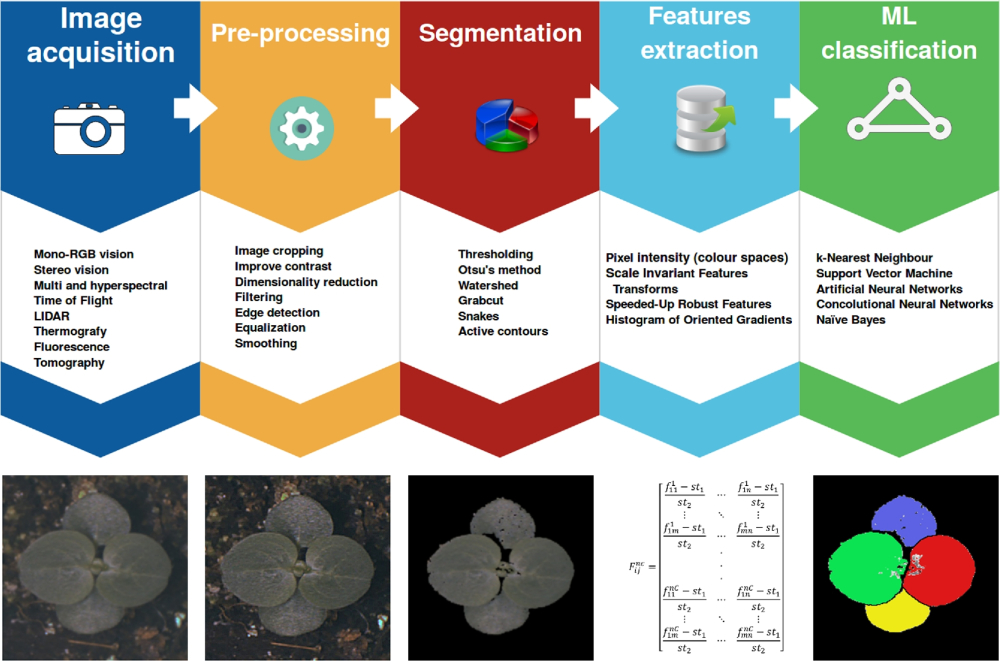
\includegraphics[width=\linewidth]{img/biblio/keys-steps}
        \caption{Étapes clés de l'analyse d'images agronomiques}
        \label{fig:03-keys-steps}
    \end{figure}
    \vfill
    
    Ainsi, ce chapitre est structuré en 5 parties, reprenant ces étapes clés de l'analyse d'image : les différents systèmes d'acquisition, les pré-traitements, la segmentation, l'extraction des paramètres et les méthodes de classification. Finalement, la conclusion permettra de synthétiser les orientations choisies durant cette thèse selon les avantages et inconvénients de chacune des méthodes par rapport au cahier des charges initial. 
    
    % modern machine learning opperate with large hight quality dataset, which together with appopriate computation ressources, motivate the design of rich functions spaces with the capacity to interpolate over data point
    
    % "Symmetry, as wide or narrow as you may define its meaning, is one idea by which man through the ages has tried to comprehend and create order, beauty, and perfection." and that was a quote from Hermann Weyl, a German mathematician who was born in the late 19th century. 
    
    \newpage
    \section{Systèmes d'imagerie}
    
    \par Pour construire un outil de vision par ordinateur, il faut comprendre comment se forment les images numériques. Un capteur en contraste noir et blanc fonctionne en estimant la quantité de photons qui frappent chaque pixel dans un laps de temps donné. Une image peut être vue comme une matrice bidimensionnelle de pixels. Ainsi, le système optique intègre donc le spectre de la lumière sur une certaine plage (380-780 pour le spectre visible) que l'on peut aussi écrire $Luminance = \int_{380}^{780} f(\lambda) d\lambda$ transformant le spectre visible $\mathbb{R}^\infty \rightarrow \mathbb{R}$.
    
    \vfill
    \begin{figure}[H]
        \centering
        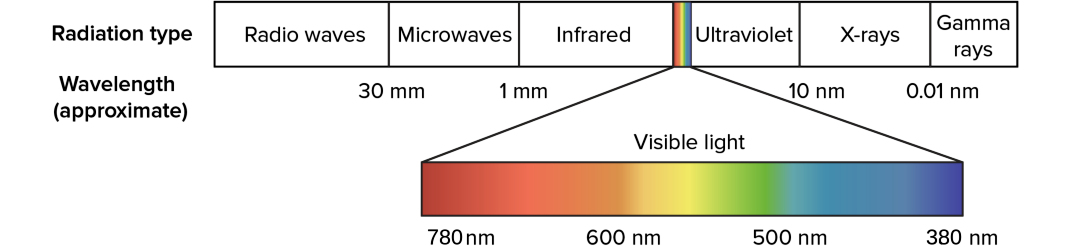
\includegraphics[width=0.7\linewidth]{img/biblio/wavelength}
        \caption{Spectre électromagnétique et spectre visible}
        \label{fig:03-wavelength}
    \end{figure}
    \vfill
    
    Pour acquérir une image, on peut utiliser un capteur CCD (Charge-Coupled Device) ou un CMOS (Complementary Metal Oxide Semiconductor). Ces éléments sont composés d'une matrice de photosites (semi-conducteurs photosensibles). Ces derniers convertissent l'information lumineuse reçue en tension électrique (analogique) exprimée en volts, puis en un nombre entier à travers un convertisseur analogique-numérique (CAN). Notons que les valeurs numériques ont une précision limitée, i.e. l'information est encodée sur un nombre de bit fixe. Avant d'arriver à la matrice de détection, la lumière passe par un système optique, composé d'une ou plusieurs lentilles et d'un filtre pour limiter la plage d'intégration (visible), tel que représenté ci-dessous (figure \ref{fig:03-image-formation}).
    
    \vfill
    \begin{figure}[H]
        \centering
        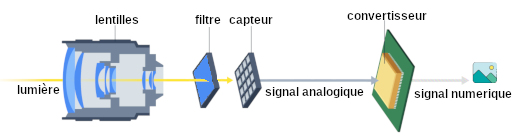
\includegraphics[width=0.7\linewidth]{img/biblio/image-formation}
        \caption{Les différents composants d'une caméra}
        \label{fig:03-image-formation}
    \end{figure}
    \vfill
    
    %Des capteurs nommés Charge-Coupled Device (CCD) sont composés d'une matrice de détecteurs sensible à la lumière et qui sont associés à un système électronique. Ce dernier convertit pour chacun de ces détecteurs l'information lumineuse reçue en tension électrique, exprimée en volts, puis en un nombre. L'ensemble des valeurs acquises par ces détecteurs constitue l'image.
    
    Dans un système optique, il y a quatre facteurs importants dans la formation de l'image : la distance focale, l'ouverture, le gain et le temps d'intégration. La combinaison de ces trois derniers facteurs contrôle la luminosité moyenne de l'image que l'on appelle également ``le triangle d'exposition''. Grâce à certaines heuristiques, le meilleur équilibre du triangle d'exposition peut être défini. Chaque constructeur de caméra ou d'appareil photo propose une méthode propriétaire embarquée dans l'appareil pour effectuer un ajustement automatique du triangle d'exposition.
    
    \newpage
    \paragraph{La distance focale} : Exprimée en mm, elle représente la distance entre le centre optique et la surface du capteur. Plus la longueur focale est courte, plus l'angle d'observation est large et vice-versa. Par exemple, un objectif de \SI{8}{mm} peut avoir un champ visuel de 110° et un objectif de \SI{50}{mm} peut avoir un champ visuel de 32°. Comme l'ouverture, la focale influence la profondeur de champ. Plus la focale est importante, plus la profondeur de champ est faible. Cela avantage les petits capteurs car à champ de vision équivalent, plus le capteur est petit, plus la focale est petite.
    
    \vspace{-0.2em}
    \begin{figure}[H]
        \centering
        \source{\href{https://fr.nikon.ca/learn-and-explore/a/tips-and-techniques/comprendre-la-longueur-focale.html}{fr.nikon.ca}}
        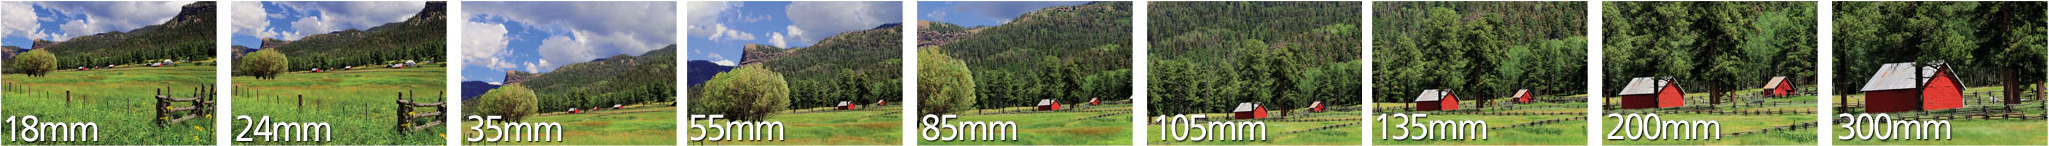
\includegraphics[width=\linewidth]{img/biblio/camera-focal}
        \caption{Effet de la longueur de la focale sur le champ de vision}
        \label{fig:03-camera-focal}
    \end{figure}
    
    \vspace{-0.5em}
    \paragraph{L'ouverture} : C'est le diamètre d'ouverture du diaphragme de l'objectif. Par exemple, l'objectif peut avoir un diamètre de \SI{70}{mm} mais seulement \SI{5}{mm} peuvent collecter la lumière. Une grande ouverture de l'objectif laissera entrer beaucoup de lumière, mais la profondeur de champ sera plus faible, ce qui signifie que seule une petite gamme de distances sera mise au point. Une grande profondeur de champ, donc une petite ouverture est préférable pour la perception robotique, car nous voulons capturer autant de détails que possibles dans la scène.
    
    \begin{figure}[H]
        \centering
        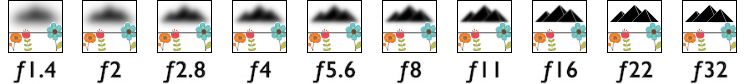
\includegraphics[width=\linewidth]{img/biblio/camera-apperture}
        \caption{Effet de l'ouverture sur la profondeur de vision}
        \label{fig:03-camera-apperture}
    \end{figure}
    
    \vspace{-0.5em}
    \paragraph{Le gain} : Ce paramètre contrôle la luminosité de l'image. Le niveau de tension mesuré par pixel peut être amplifié par un facteur, appelé gain ou sensibilité ISO. Un gain plus élevé signifie une image plus lumineuse et vice-versa. L'amplification du signal induit également l'amplification du bruit. Il faut donc trouver un équilibre entre l'amplification et le bruit. En condition de faible luminosité, ce paramètre est essentiel pour distinguer les objets.
    
    \begin{figure}[H]
        \centering
        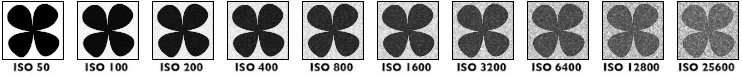
\includegraphics[width=\linewidth]{img/biblio/camera-iso}
        \caption{Effet du gain sur le bruit de l'image}
        \label{fig:03-camera-iso}
    \end{figure}
    
    \vspace{-0.5em}
    \paragraph{Temps d'intégration}: Il s'agit de la durée, en secondes, pendant laquelle le capteur collecte la lumière. La tension mesurée sera la somme de tous les photons collectés pendant le temps d'intégration. Une vitesse d'obturation plus longue laissera entrer plus de lumière, mais rendra tout mouvement flou.  Ce phénomène est communément appelé le ``flou de bougé''.
    
    \begin{figure}[H]
        \centering
        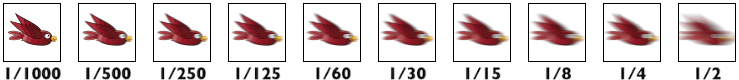
\includegraphics[width=\linewidth]{img/biblio/camera-integration}
        \caption{Effet du temps d'intégration (en seconde) sur le flou de bougé}
        \label{fig:03-camera-integration}
    \end{figure}
    
    \newpage
    \subsection{Percevoir la couleur}
    \label{sec:percevoir-couleur}
    
    Pour percevoir la couleur plutôt que les niveaux de gris, le capteur doit être capable de séparer la lumière en différents domaines spectraux ; c'est-à-dire de transformer le spectre visible de $\mathbb{R}^\infty \rightarrow \mathbb{R}^{N}$, avec $N$ le nombre de couleurs, généralement $3$ pour $RGB$  (Red, Green, Blue). L'image est alors représentée comme un tableau à trois dimensions de taille $Largeur \times Hauteur \times N$. Chaque couche de couleur intègre une tranche du spectre (domaine spectral). Plusieurs approches sont possibles :
    
    \paragraph{Filtre colorimétrique}
    L'approche la plus courante et la moins coûteuse est de disposer les pixels selon un motif, tel que le filtre de ``Bayer'', comme illustré ci-dessous (figure \ref{fig:03-bayer-filter}). Les filtres de Bayer disposent deux fois plus de pixels verts que de pixels rouges ou bleus. Ce qui signifie que certaines couleurs seront plus bruitées que d'autres, ici rouge et bleu. Généralement, le bleu est naturellement moins présent en extérieur et donc plus difficile à estimer. Mais il existe différents types de filtres et certains se concentrent davantage sur le bleu tel que les filtres RGBE \cite{miao2004generic}. Dans ce cas, le canal bleu n'est pas le plus bruité. Le désavantage de ces filtres est qu'ils diminuent la résolution physique. On a alors recours à un algorithme d'interpolation pour estimer les couleurs manquantes (Demosaicing) \cite{rathi2021convolution}. Certaines méthodes de demosaicing peuvent partiellement corriger le bruit associé à une couleur \cite{tan2014green} en se basant sur la plus présente, par exemple sur le vert pour les filtres de Bayer.
    
    \begin{figure}[H]
        \centering
        %{\scriptsize (source : wikipedia.fr) } \\
        %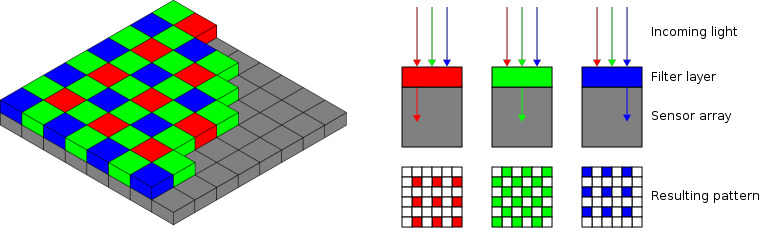
\includegraphics[width=0.6\linewidth]{img/biblio/bayer-filter}
        \begin{tikzpicture}[>=stealth', tip/.style={->,shorten >=0.007pt}]
	\begin{scope}[scale=0.8, xshift=10]
		\begin{scope}[yshift=-10,every node/.append style={yslant=0.5,xslant=-1},yslant=0.5,xslant=-1]
			\fill[black!5] (0,0) rectangle (2.4,2.4);
			\draw[step=4mm, black] (0,0) grid (2.4,2.4);
			\fill[black!35] (0.05,2.05) rectangle (0.35,2.35);
			\fill[black!35] (0.45,2.05) rectangle (0.75,2.35);
			\fill[black!35] (0.85,2.05) rectangle (1.15,2.35);
			\fill[black!35] (1.25,2.05) rectangle (1.55,2.35);
			\fill[black!35] (1.65,2.05) rectangle (1.95,2.35);
			\fill[black!35] (2.05,2.05) rectangle (2.35,2.35);
			
			\fill[black!35] (0.05,1.65) rectangle (0.35,1.95);
			\fill[black!35] (0.45,1.65) rectangle (0.75,1.95);
			\fill[black!35] (0.85,1.65) rectangle (1.15,1.95);
			\fill[black!35] (1.25,1.65) rectangle (1.55,1.95);
			\fill[black!35] (1.65,1.65) rectangle (1.95,1.95);
			\fill[black!35] (2.05,1.65) rectangle (2.35,1.95);
			
			\fill[black!35] (0.05,1.25) rectangle (0.35,1.55);
			\fill[black!35] (0.45,1.25) rectangle (0.75,1.55);
			\fill[black!35] (0.85,1.25) rectangle (1.15,1.55);
			\fill[black!35] (1.25,1.25) rectangle (1.55,1.55);
			\fill[black!35] (1.65,1.25) rectangle (1.95,1.55);
			\fill[black!35] (2.05,1.25) rectangle (2.35,1.55);
			
			\fill[black!35] (0.05,0.85) rectangle (0.35,1.15);
			\fill[black!35] (0.45,0.85) rectangle (0.75,1.15);
			\fill[black!35] (0.85,0.85) rectangle (1.15,1.15);
			\fill[black!35] (1.25,0.85) rectangle (1.55,1.15);
			\fill[black!35] (1.65,0.85) rectangle (1.95,1.15);
			\fill[black!35] (2.05,0.85) rectangle (2.35,1.15);
			
			\fill[black!35] (0.05,0.45) rectangle (0.35,0.75);
			\fill[black!35] (0.45,0.45) rectangle (0.75,0.75);
			\fill[black!35] (0.85,0.45) rectangle (1.15,0.75);
			\fill[black!35] (1.25,0.45) rectangle (1.55,0.75);
			\fill[black!35] (1.65,0.45) rectangle (1.95,0.75);
			\fill[black!35] (2.05,0.45) rectangle (2.35,0.75);
			
			\fill[black!35] (0.05,0.05) rectangle (0.35,0.35);
			\fill[black!35] (0.45,0.05) rectangle (0.75,0.35);
			\fill[black!35] (0.85,0.05) rectangle (1.15,0.35);
			\fill[black!35] (1.25,0.05) rectangle (1.55,0.35);
			\fill[black!35] (1.65,0.05) rectangle (1.95,0.35);
			\fill[black!35] (2.05,0.05) rectangle (2.35,0.35);
			\node (F) at (1.2,-0.4) {\small Sensor Array};
		\end{scope}
		
		\begin{scope}[yshift=0,every node/.append style={yslant=0.5,xslant=-1},yslant=0.5,xslant=-1]
			\fill[black!5] (0,0) rectangle (2.4,2.4);
			\draw[step=4mm, black] (0,0) grid (2.4,2.4); 
			\draw[black,thick] (0,0) rectangle (2.4,2.4);
			
			\fill[blue] (0.05,2.05) rectangle (0.35,2.35);
			\fill[green] (0.45,2.05) rectangle (0.75,2.35);
			\fill[blue] (0.85,2.05) rectangle (1.15,2.35);
			\fill[green] (1.25,2.05) rectangle (1.55,2.35);
			\fill[blue] (1.65,2.05) rectangle (1.95,2.35);
			\fill[green] (2.05,2.05) rectangle (2.35,2.35);
			
			\fill[green] (0.05,1.65) rectangle (0.35,1.95);
			\fill[red] (0.45,1.65) rectangle (0.75,1.95);
			\fill[green] (0.85,1.65) rectangle (1.15,1.95);
			\fill[red] (1.25,1.65) rectangle (1.55,1.95);
			\fill[green] (1.65,1.65) rectangle (1.95,1.95);
			\fill[red] (2.05,1.65) rectangle (2.35,1.95);
			
			\fill[blue] (0.05,1.25) rectangle (0.35,1.55);
			\fill[green] (0.45,1.25) rectangle (0.75,1.55);
			\fill[blue] (0.85,1.25) rectangle (1.15,1.55);
			\fill[green] (1.25,1.25) rectangle (1.55,1.55);
			\fill[blue] (1.65,1.25) rectangle (1.95,1.55);
			\fill[green] (2.05,1.25) rectangle (2.35,1.55);
			
			\fill[green] (0.05,0.85) rectangle (0.35,1.15);
			\fill[red] (0.45,0.85) rectangle (0.75,1.15);
			\fill[green] (0.85,0.85) rectangle (1.15,1.15);
			\fill[red] (1.25,0.85) rectangle (1.55,1.15);
			\fill[green] (1.65,0.85) rectangle (1.95,1.15);
			\fill[red] (2.05,0.85) rectangle (2.35,1.15);
			
			\fill[blue] (0.05,0.45) rectangle (0.35,0.75);
			\fill[green] (0.45,0.45) rectangle (0.75,0.75);
			\fill[blue] (0.85,0.45) rectangle (1.15,0.75);
			\fill[green] (1.25,0.45) rectangle (1.55,0.75);
			\fill[blue] (1.65,0.45) rectangle (1.95,0.75);
			\fill[green] (2.05,0.45) rectangle (2.35,0.75);
			
			\fill[green] (0.05,0.05) rectangle (0.35,0.35);
			\fill[red] (0.45,0.05) rectangle (0.75,0.35);
			\fill[green] (0.85,0.05) rectangle (1.15,0.35);
			\fill[red] (1.25,0.05) rectangle (1.55,0.35);
			\fill[green] (1.65,0.05) rectangle (1.95,0.35);
			\fill[red] (2.05,0.05) rectangle (2.35,0.35);
			
			\node (F) at (1.2,2.7) {\small Filter Layer};
		\end{scope}
	\end{scope}
	
	\begin{scope}[yshift=-10, xshift=90, scale=0.5]
		\fill[black!5] (0,0) rectangle (2.4,2.4);
		
		\fill[red] (0.4,1.6) rectangle (0.8,2.0);
		\fill[red] (1.2,1.6) rectangle (1.6,2.0);
		\fill[red] (2.0,1.6) rectangle (2.4,2.0);
		\fill[red] (0.4,0.8) rectangle (0.8,1.2);
		\fill[red] (1.2,0.8) rectangle (1.6,1.2);
		\fill[red] (2.0,0.8) rectangle (2.4,1.2);
		\fill[red] (0.4,0.0) rectangle (0.8,0.4);
		\fill[red] (1.2,0.0) rectangle (1.6,0.4);
		\fill[red] (2.0,0.0) rectangle (2.4,0.4);
		
		\draw[step=4mm, black] (0,0) grid (2.4,2.4); 
		\draw[black,thick] (0,0) rectangle (2.4,2.4);
		
		\fill[black!35] (0,2.8) rectangle (2.4,4);
		\draw[black,thick] (0,2.8) rectangle (2.4,4);
		\fill[red] (0,4) rectangle (2.4,4.5);
		\draw[black,thick] (0,4) rectangle (2.4,4.5);
		
		\draw[->, blue,line width=0.5mm] (1.2,6) to (1.2,4.5);
		\draw[->, green,line width=0.5mm] (1.8,6) to (1.8,4.5);
		\draw[->, red,line width=0.5mm] (0.6,6) to (0.6,3.1);
	\end{scope}
	
	\begin{scope}[yshift=-10, xshift=130, scale=0.5]
		\fill[black!5] (0,0) rectangle (2.4,2.4);
		
		\fill[green] (0.4,2.0) rectangle (0.8,2.4);
		\fill[green] (1.2,2.0) rectangle (1.6,2.4);
		\fill[green] (2.0,2.0) rectangle (2.4,2.4);
		\fill[green] (0.0,1.6) rectangle (0.4,2.0);
		\fill[green] (0.8,1.6) rectangle (1.2,2.0);
		\fill[green] (1.6,1.6) rectangle (2.0,2.0);
		\fill[green] (0.4,1.2) rectangle (0.8,1.6);
		\fill[green] (1.2,1.2) rectangle (1.6,1.6);
		\fill[green] (2.0,1.2) rectangle (2.4,1.6);
		\fill[green] (0.0,0.8) rectangle (0.4,1.2);
		\fill[green] (0.8,0.8) rectangle (1.2,1.2);
		\fill[green] (1.6,0.8) rectangle (2.0,1.2);
		\fill[green] (0.4,0.4) rectangle (0.8,0.8);
		\fill[green] (1.2,0.4) rectangle (1.6,0.8);
		\fill[green] (2.0,0.4) rectangle (2.4,0.8);
		\fill[green] (0.0,0.0) rectangle (0.4,0.4);
		\fill[green] (0.8,0.0) rectangle (1.2,0.4);
		\fill[green] (1.6,0.0) rectangle (2.0,0.4);
		
		\draw[step=4mm, black] (0,0) grid (2.4,2.4); 
		\draw[black,thick] (0,0) rectangle (2.4,2.4);
		
		\fill[black!35] (0,2.8) rectangle (2.4,4);
		\draw[black,thick] (0,2.8) rectangle (2.4,4);
		\fill[green] (0,4) rectangle (2.4,4.5);
		\draw[black,thick] (0,4) rectangle (2.4,4.5);
		
		\draw[->, red,line width=0.5mm] (0.6,6) to (0.6,4.5);
		\draw[->, blue,line width=0.5mm] (1.2,6) to (1.2,4.5);
		\draw[->, green,line width=0.5mm] (1.8,6) to (1.8,3.1);
	\end{scope}
	
	\begin{scope}[yshift=-10, xshift=170, scale=0.5]
		\fill[black!5] (0,0) rectangle (2.4,2.4);
		
		\fill[blue] (0.0,2.0) rectangle (0.4,2.4);
		\fill[blue] (0.8,2.0) rectangle (1.2,2.4);
		\fill[blue] (1.6,2.0) rectangle (2.0,2.4);
		\fill[blue] (0.0,1.2) rectangle (0.4,1.6);
		\fill[blue] (0.8,1.2) rectangle (1.2,1.6);
		\fill[blue] (1.6,1.2) rectangle (2.0,1.6);
		\fill[blue] (0.0,0.4) rectangle (0.4,0.8);
		\fill[blue] (0.8,0.4) rectangle (1.2,0.8);
		\fill[blue] (1.6,0.4) rectangle (2.0,0.8);
		
		\draw[step=4mm, black] (0,0) grid (2.4,2.4); 
		\draw[black,thick] (0,0) rectangle (2.4,2.4);
		
		\fill[black!35] (0,2.8) rectangle (2.4,4);
		\draw[black,thick] (0,2.8) rectangle (2.4,4);
		\fill[blue] (0,4) rectangle (2.4,4.5);
		\draw[black,thick] (0,4) rectangle (2.4,4.5);
		
		\draw[->, red,line width=0.5mm] (0.6,6) to (0.6,4.5);
		\draw[->, green,line width=0.5mm] (1.8,6) to (1.8,4.5);
		\draw[->, blue,line width=0.5mm] (1.2,6) to (1.2,3.1);
	\end{scope}
	
	\node (I) at (9,2.30) {\scriptsize Incomming Light};
	\node (F) at (9,1.70) {\scriptsize Filter Layer};
	\node (S) at (9,1.20) {\scriptsize Sensor Array};
	\node (R) at (9,0.50) {\scriptsize Resulting Pattern};
	\node (R) at (11.5,0.50) {\scriptsize RGB Image};
	\node (R) at (10.3,-0.25) {\scriptsize Demosaicing};
	
	\draw[->] (9,0.3) to (9,0.0) to (11.5,0.0) to (11.5,0.3);
	
	\begin{scope}[yshift=25, xshift=310]
		\begin{scope}[yshift=0, xshift=0, scale=0.5]
			\fill[red, fill opacity=.7] (0,0) rectangle (2.4,2.4);
			\draw[step=4mm, black] (0,0) grid (2.4,2.4); 
			\draw[black,thick] (0,0) rectangle (2.4,2.4);
		\end{scope}
		\begin{scope}[yshift=3, xshift=3, scale=0.5]
			\fill[green, fill opacity=.7] (0,0) rectangle (2.4,2.4);
			\draw[step=4mm, black] (0,0) grid (2.4,2.4); 
			\draw[black,thick] (0,0) rectangle (2.4,2.4);
		\end{scope}
		\begin{scope}[yshift=6, xshift=6, scale=0.5]
			\fill[blue, fill opacity=.7] (0,0) rectangle (2.4,2.4);
			\draw[step=4mm, black] (0,0) grid (2.4,2.4); 
			\draw[black,thick] (0,0) rectangle (2.4,2.4);
		\end{scope}
	\end{scope}
\end{tikzpicture}
        \caption{Filtre de Bayer}
        \label{fig:03-bayer-filter}
    \end{figure}
    
    \paragraph{Diviser la lumière incidente}
    
    Parmi les techniques de dispersion (réseaux de diffraction, réflexion, \dots) de la lumière dans un capteur optique, plusieurs prismes peuvent être utilisés pour diviser la lumière incidente vers des capteurs physiquement séparés qui absorbent les longueurs d'onde différentes (figure \ref{fig:03-prism-sensors}). L'avantage de cette technique est d'obtenir des images couleurs de haute qualité avec une résolution physique complète. Les capteurs peuvent être exposés pendant des temps différents pour gérer le bruit efficacement. La difficulté d'alignement précis des prismes \cite{galo2006registration} rend cette technologie coûteuse.
    
    \begin{figure}[H]
        \centering
        %{\scriptsize (source : \href{https://www.vision-doctor.com/en/line-scan-cameras/colour-line-scan-cameras.html}{vision-doctor.com}) } \\
        %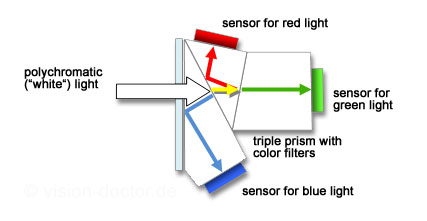
\includegraphics[width=0.4\linewidth]{img/biblio/prism-sensors-old}
        %\source{\cite{Pan2017}}
        %\rotatebox{90}{\scriptsize (source : \cite{Pan2017})}
        %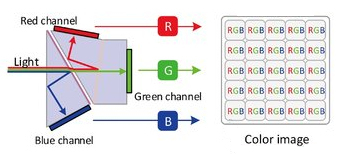
\includegraphics[width=0.5\linewidth]{img/biblio/prism-sensors}
        

\begin{tikzpicture}[>=stealth', tip/.style={->,shorten >=0.007pt}]

    \coordinate (A) at (0.4,1.5);
    \coordinate (B) at (1.9,-0.75);
    \coordinate (C) at (2.8,0.75);
    
    \filldraw [thick, even odd rule, black!35] (3.5,0.75)  coordinate (GeneralStart) -- (C) -- (A) -- (0.35,-2) -- (B) -- (3.5,-0.75) -- cycle;
    \draw[thick] (3.5,0.75) -- (C) -- (A) -- (0.35,-2) -- (B) -- (3.5,-0.75) -- cycle;
    \draw[thick, red, opacity=0.8] (B) -- (C);
    \draw[thick, blue, opacity=0.8] (A) -- (B);
    
    \draw[->, blue,line width=0.5mm] (-2,-0.05) to (1.25,-0.05) to (0.39,-0.6) to (1.0,-1.46);
    \draw[->, green,line width=0.5mm] (-2,0) to (3.5,0);
    \draw[->, red,line width=0.5mm] (-2,0.05) to (2.2,0.05) to (0.95, 0.7) to (1.2,1.2);
    
    \node (I) at (-0.9,0.30) {\scriptsize Incomming Light};
    \node (R) at (1.7,1.5) {\scriptsize Red};
    \node (G) at (4.15,-0.2) {\scriptsize Green};
    \node (B) at (1.5,-1.7) {\scriptsize Blue};
    \node (Img) at (9.5,-0.8) {\scriptsize RGB Image};
    
    \draw[fill=blue, rotate around={38:(1.0,-1.6)}] (0.55,-1.5) rectangle (1.6,-1.65);
    \draw[fill=green] (3.5,-0.5) rectangle (3.65,0.5);
    \draw[fill=red, rotate around={-18:(1.1,1.15)}] (0.6,1.27) rectangle (1.6,1.42);
    
    \draw (1.3,-1.26) to (5.0,-1.26) to (5.0,0.0);
    \draw[->] (3.65,0) to (5.5,0.0);
    \draw (1.64,1.15) to (5.0, 1.15) to (5.0,0.0);
    
    \begin{scope}[yshift=22, xshift=170, scale=0.5]
        \fill[red] (0,0) rectangle (2.4,2.4);
        \draw[step=4mm, black] (0,0) grid (2.4,2.4); 
        \draw[black,thick] (0,0) rectangle (2.4,2.4);
    \end{scope}
    \begin{scope}[yshift=-18, xshift=170, scale=0.5]
        \fill[green] (0,0) rectangle (2.4,2.4);
        \draw[step=4mm, black] (0,0) grid (2.4,2.4); 
        \draw[black,thick] (0,0) rectangle (2.4,2.4);
    \end{scope}
    \begin{scope}[yshift=-58, xshift=170, scale=0.5]
        \fill[blue] (0,0) rectangle (2.4,2.4);
        \draw[step=4mm, black] (0,0) grid (2.4,2.4); 
        \draw[black,thick] (0,0) rectangle (2.4,2.4);
    \end{scope}
    
    \draw (7.5,-1.26) to (8.0,-1.26) to (8.0,0.0);
    \draw[->] (7.5,0) to (8.5,0.0);
    \draw (7.5,1.15) to (8.0, 1.15) to (8.0,0.0);
    
    \begin{scope}[yshift=-10, xshift=250]
        \begin{scope}[yshift=0, xshift=0, scale=0.5]
            \fill[red, fill opacity=.7] (0,0) rectangle (2.4,2.4);1
            \draw[step=4mm, black] (0,0) grid (2.4,2.4); 
            \draw[black,thick] (0,0) rectangle (2.4,2.4);
        \end{scope}
        \begin{scope}[yshift=3, xshift=3, scale=0.5]
            \fill[green, fill opacity=.7] (0,0) rectangle (2.4,2.4);
            \draw[step=4mm, black] (0,0) grid (2.4,2.4); 
            \draw[black,thick] (0,0) rectangle (2.4,2.4);
        \end{scope}
        \begin{scope}[yshift=6, xshift=6, scale=0.5]
            \fill[blue, fill opacity=.7] (0,0) rectangle (2.4,2.4);
            \draw[step=4mm, black] (0,0) grid (2.4,2.4); 
            \draw[black,thick] (0,0) rectangle (2.4,2.4);
        \end{scope}
    \end{scope}

\end{tikzpicture}
        \caption{Triple prismes pour diviser la lumière incidente}
        \label{fig:03-prism-sensors}
    \end{figure}
    
    \newpage
    \subsection{Des capteurs multispectraux}
    
    Nous avons vu précédemment que la première approche a le désavantage de réduire la résolution physique, tandis que la seconde est coûteuse et il devient impossible pour les deux méthodes d'obtenir efficacement plus de couleurs (infrarouge, ultraviolet, \dots). Pour pallier ces désavantages, d'autres dispositifs (multispectraux) sont apparus : les systèmes d'acquisition d'images multispectrales qui permettent d'extraire un certain nombre de propriétés sur les surfaces observées \cite{Qiu:2018:10.25165}. Leurs utilisations se sont diversifiées pour caractériser l'état sanitaire des cultures, la texture des sols, le stress hydrique, ou encore la présence de végétation.
    
    \paragraph{Filtre rotatif}
    
    Ce type de dispositif, développé au début des années 2000 \cite{vioix2004}, associe un système optique à une roue portant les différents filtres colorimétriques. Plusieurs acquisitions sont effectuées pour obtenir les différentes couleurs. L'avantage de ce dispositif est d'être très peu coûteux tout en fournissant des images de grandes résolutions. Mais faire tourner le filtre engendre des problèmes de recalage des images mono-modes d'une même scène. Ce dispositif ne peut donc pas être utilisé efficacement en conditions extérieures en particulier en présence de mouvement.
    
    \begin{figure}[H]
        \centering
        {\scriptsize (source : \cite{vioix2004}) } \\
        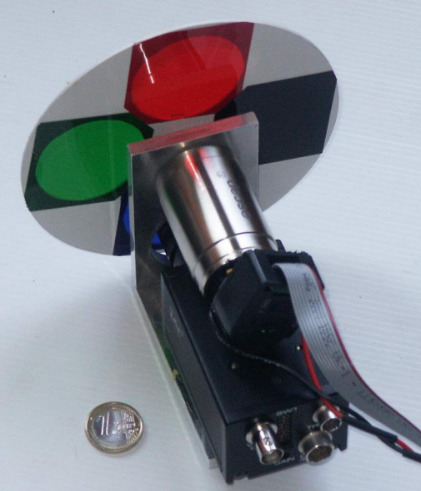
\includegraphics[height=3cm]{img/biblio/spinning-color}
        \caption{Filtre rotatif à 4 bandes spectrales : bleu, vert, rouge et infrarouge}
        \label{fig:03-spinning-color}
    \end{figure}
    
    \paragraph{Capteurs multiples}
    
    Une autre solution est d'utiliser plusieurs caméras disposées en damier. Chaque caméra dispose d'un filtre permettant de percevoir une section différente du spectre. C'est le cas du dispositif développé par HYPHEN pour l'acquisition d'images depuis un drone aérien, et qui a été utilisé durant cette thèse (Cf. détails en chapitre \ref{chap:mat-and-data}). Cette solution a l'avantage d'avoir des temps d'acquisition très courts, contrairement au dispositif proposé par \cite{vioix2004} et peut également être utilisé en mouvement. Cependant, du fait de la différence de position des capteurs sur le système d'imagerie, leurs champs de vision ne sont pas identiques. Ceci implique l'utilisation d'algorithmes complexes pour superposer les images mono-modes. À cet effet, un algorithme spécifique est proposé dans ce manuscrit (section \ref{chap:image-registration}).
    
    \paragraph{Vers l'hyperspectral}
    
    D'autres solutions permettent d'obtenir des images dites hyperspectrales, c'est-à-dire un découpage plus fin du spectre électromagnétique. Par exemple $\mathbb{R}^\infty \rightarrow \mathbb{R}^{100}$, on parle alors d'hyper-cube. La solution proposée par le consortium PEAD du challenge RoSE, repose sur un spectromètre imageur par tomographie (CTIS \cite{descour1995computed}) développée par CarbonBee. L'imagerie hyperspectrale présente de nombreux avantages et a de nombreux domaines d'application (agriculture, médecine, minéralogie, surveillance, astronomie, chimie, etc). Son prix est encore élevé ce qui limite fortement son utilisation. Ce dispositif permet de définir les longueurs d'onde les plus discriminantes pour un sujet donné, de manière à orienter le choix de capteurs multispectraux, plus abordables. Nous verrons plus tard, que le dispositif multispectral utilisé dans cette thèse repose sur les travaux de \cite{louar2016}.
    
    \newpage
    %\subsection{En agriculture}
    %
    %En agriculture, de nombreux capteurs d'image ont été étudiés. 
    %
    %\begin{table}[H]
    %	\begin{tabularx}{\linewidth}{l X X}
    %		\hline
    %		\textbf{Capteurs} & \textbf{Avantage}  & \textbf{Désavantage} \\
    %		\hline
    %			Stéréo vision &
    %			Faible coût - Haute résolution - Adapté aux drones &
    %			Calcul lourd - Sensible à la lumière ambiante - Soumis à une texture uniforme \\
    %			\hline
    %			Lidar/capteur laser &
    %			Longue plage de mesure - Adapté à la classification spatiale - L'information spectrale peut être extraite de la réflexion - Adapté aux drones &
    %			Coût élevé - Information limitée sur les occlusions et les ombres \\
    %			\hline
    %			Caméra à distance &
    %			Fournit des images de profondeur à traiter &
    %			Faible résolution - Sensible à la lumière ambiante - Courte plage de mesure \\
    %			\hline
    %			Capteur spectral &
    %			Applications commerciales étendues et maturité technologique &
    %			Petite région de mesure - Interférence de fond \\
    %			\hline
    %			Caméra spectrale &
    %			Abondance d'information spectrale - Suppression de l'interférence de fond Suppression des interférences de fond - Convient aux drones &
    %			Coût élevé - Grandes données d'image et calculs lourds - Sensible aux conditions ambiantes \\
    %			\hline
    %			Thermographie &
    %			Grande zone de mesure - Suppression des interférences de fond - Convient aux drones &
    %			Sensible aux conditions ambiantes - Nécessite un étalonnage important \\
    %			\hline
    %		  	Capteur de fluorescence &
    %		  	Sensible à la chlorophylle et au stress hydrique &
    %		  	Petit champ de vision - Nécessite un éclairage intensif \\
    %		  	\hline
    %		  	Capteur ultrasonique &
    %		  	Faible coût - Fréquence d'échantillonnage élevée - Traitement facile des données &
    %		  	Courte plage de mesure - Sensible à la surface \\
    %		  	\hline
    %			Thermomètre &
    %			Faible coût - Imperméable à la lumière du soleil &
    %			Affecté par la température ambiante - Interférences de fond avec le sol \\
    %		\hline
    %	\end{tabularx}
    %	\caption{Avantages et inconvénients des capteurs courants mis en œuvre}
    %\end{table}
    
    \newpage
    \section{Prétraitement}
    
    Le système optique engendre par nature des distorsions de l'image. Il existe plusieurs sources d'erreurs qui peuvent amener à des déformations géométriques et/ou colorimétriques. Au niveau colorimétrique, l'objectif du prétraitement des images est d'améliorer le contraste et d'éliminer le bruit afin de mettre en valeur les objets d'intérêt dans une image donnée. Les pré-traitements permettent aussi de stabiliser certaines méthodes de segmentation ainsi que la qualité de l'extraction des caractéristiques. Les sous-sections suivantes expliquent et présentent les corrections possibles.
    
    \subsection{Correction géométrique}
    \label{sec:lens-correction}
    
    Les premières déformations sont issues de la lentille de l'appareil et de l'alignement du capteur à cette dernière. Ces déformations peuvent se modéliser mathématiquement. Trois sources d'erreurs sont à prendre en considération :
    
    \begin{itemize}
        \item \textbf{Distorsion radiale :} La distorsion radiale se produit lorsque les rayons lumineux se courbent plus près des bords d'une lentille qu'ils ne le font en son centre optique. Plus la lentille est petite, plus la distorsion est importante. La distorsion peut être positive (barrel) ou négative (pincushion)
        \item \textbf{Distorsion tangentielle :} La distorsion tangentielle corrige les inclinaisons du plan de l'image (capteur) après une distorsion radiale.
        \item \textbf{Distorsion prismatique :} La distorsion à prisme mince est due à une légère inclinaison de la lentille ou du réseau de capteurs d'images et provoque des distorsions radiales et tangentielles supplémentaires.
    \end{itemize}
    
    \par En résumé, les différentes distorsions se cumulent et constituent le modèle de distorsion (figure \ref{fig:03-distorsion-models}). Pour rectifier les déformations d'une image, il faut inverser le modèle, mais il n'existe pas d'expression de forme close pour estimer ce mappage inverse. En pratique, l'évaluation est effectuée par un processus de table de recherche. Dans l'ensemble, ce modèle de caméra avec distorsion de l'objectif comprend jusqu'à onze paramètres intrinsèques en plus des paramètres extrinsèques, avec six degrés de liberté. % Il existe plusieurs outils pour estimer ce modèle de correction.
    
    \begin{figure}[H]
        \centering
        \source{\cite{LIU2018119}}
        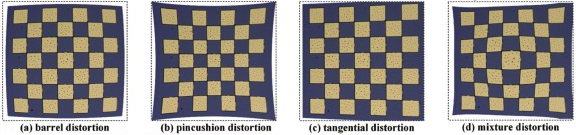
\includegraphics[width=\linewidth]{img/biblio/distorsion-models}
        \caption{Modèle de distorsion}
        \label{fig:03-distorsion-models}
    \end{figure}
    
    \par Cette correction est indispensable si l'on cherche à évaluer la distance d'un objet à l'objectif ou mesurer la taille d'objet \cite{vayssade2018spatial}. En effet, la distorsion géométrique de l'image induit une distorsion des surfaces et des distances. En l'absence de ce type d'analyse, la correction géométrique n'est pas indispensable.
    
    \newpage
    \subsection{Rehaussement d'image}
    \label{sec:correction-color}
    
    \par Le ré-haussement d'images est essentiellement un processus qui permet de faciliter l'interprétation d'une image. Ainsi, rehausser l'image, consiste entre autres à standardiser l'information, comme corriger la luminosité, l'intensité des couleurs ou à supprimer des effets de l'environnement comme l'ombre ou le bruit. %La couleur est donc la seconde source d'erreur.
    
    \subsubsection{Correction colorimétrique et radiométrique}
    
    Selon les paramètres de la caméra (triangle d'exposition), de l'illuminant et les filtres spectraux employés, la quantité de photons reçue, et donc l'estimation des couleurs de la scène peut être biaisée. Nous avons vu par exemple dans la section précédente que les filtres de Bayer sous-évalue le bleu \cite{1561853}. L'illuminant joue aussi un rôle prédominant puisqu'il change la distribution des photons émis \cite{brainard1992asymmetric}. L'objectif est alors de déterminer la couleur des objets dans des conditions d'éclairage différentes en supprimant l'effet de décalage des spectres. Les méthodes employées reposent souvent sur l'utilisation d'un dispositif d'étalonnage, on prend alors en photo le dispositif dont les couleurs sont connues a priori. Une équation permet ensuite de corriger les couleurs dans ces mêmes conditions d'acquisition afin d'obtenir des images standardisées. D'autres approches sont toutefois possibles et ne nécessitent pas de dispositif d'étalonnage \cite{color-correction, DBLP:journals/corr/abs-1802-00153}, ces méthodes ne sont pas encore utilisées en agriculture de précision.
    
    \begin{figure}[H]
        \centering
        \source{\cite{DBLP:journals/corr/abs-1802-00153}}
        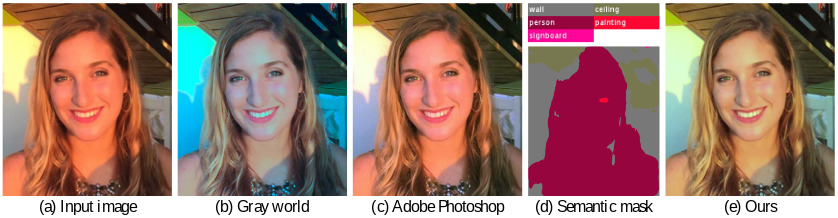
\includegraphics[width=0.7\linewidth]{img/biblio/color-consistancy}
        \caption{Correction des couleurs par apprentissage profond proposé par Afifi}
        \label{fig:03-color-consistancy}
    \end{figure}
    
    %\paragraph{Adaptative Gamma Correction} Une correction gamma non-locale peut être appliquée, on peut alors estimer l'intensité moyenne d'un pixel avec son voisinage, le but est alors de normaliser la valeur de l'intensité pour chaque pixel avec leur voisinage. Il en résulte une amélioration de l'éclairage dans les zones ombragées (sous-exposées).
    
    \vspace{-0.5em}
    \paragraph{Calibration radiométrique} La correction radiométrique suit les mêmes principes, mais permet d'obtenir des mesures de réflectance \cite{rs10020256} (figure \ref{fig:03-radiometric-correction}). La réflectance se définit comme la proportion de lumière réfléchie par la surface d'un matériau et s'exprime généralement en pourcentage. La réflectance spectrale est estimée afin de rendre la discrimination robuste aux variations d'illumination. Les indices de végétation reposent sur ces valeurs calibrées. L'étude de \cite{s21113601} permet l'estimation de la réflectance sans dispositif d'étalonnage en proxidétection.
    %https://www.mdpi.com/2072-4292/10/2/256/htm
    
    \begin{figure}[H]
        \centering
        \source{\cite{rs10020256}}
        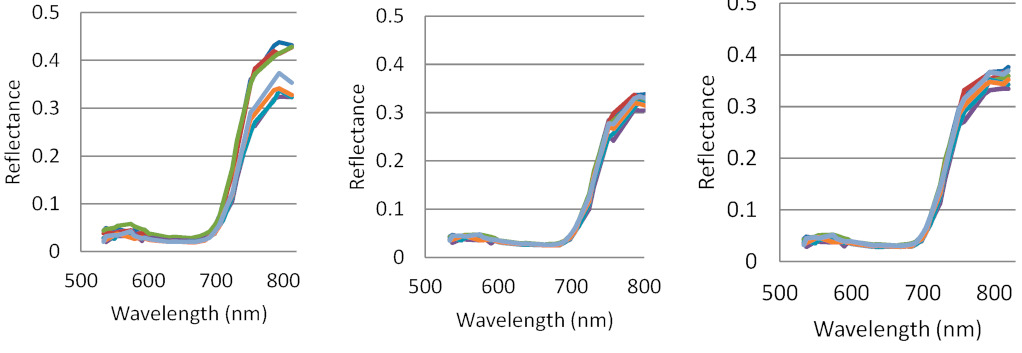
\includegraphics[width=0.7\linewidth]{img/biblio/radiometric-correction}
        \caption{Différentes corrections radiométriques proposé par Honkavaara}
        \label{fig:03-radiometric-correction}
    \end{figure}
    
    \newpage
    \subsubsection{Correction du bruit}
    
    \par De par l'environnement d'acquisition et la qualité du matériel utilisé, il peut être intéressant d'estimer et de corriger le bruit éventuel des capteurs. Le ``bruit d'image'' est l'équivalent numérique du grain des caméras analogiques. Pour les images numériques, ce bruit apparaît sous la forme de points aléatoires et peut dégrader considérablement la qualité de l'image. Le bruit augmente avec le réglage de la sensibilité de l'appareil photographique, le temps d'exposition, la température, et varie également d'un modèle d'appareil photographique à l'autre.
    
    \begin{figure}[H]
        \centering
        {\scriptsize (source: \href{https://scikit-image.org/docs/stable/auto_examples/filters/plot_denoise.html}{scikit-image.org})} \\
        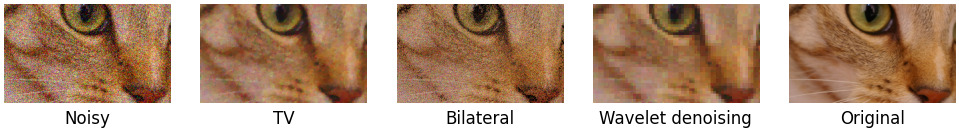
\includegraphics[width=0.7\linewidth]{img/biblio/denoising}
        \caption{Comparaison des méthodes de débruitage}
        \label{fig:03-denoising}
    \end{figure}
    
    Il n'existe pas de méthode propre à l'agriculture de précision, cependant, il existe de nombreuses méthodes générales \cite{doi:10.1137/040616024}. Les plus connues pour ce type de traitement sont les filtres bilatéraux \cite{DBLP:journals/corr/ChaudhuryD16}, les ``Non local means'', les ``Wavelet-based tresholding denoising'' \cite{hao2014wavelet}, ``Random Field Denoising'' \cite{5173526} ou encore les filtres ``Total Variation''. Pour autant, toutes ces approches sont gourmandes en temps de calcul et ne permettent pas une utilisation en temps réel. De plus supprimer le bruit d'une image peut également lisser les textures et ainsi induire à une perte d'information utile à la discrimination. Ici encore l'apprentissage profond surpasse les méthodes usuelles \cite{tian2020deep, Zamir2020MIRNet}.
    
    \subsubsection{Correction d'ombrage} La présence d'ombres est naturelle dans une scène. Une ombre portée modifie la couleur sur une partie de l'image et ajoute des ruptures de gradient. Ainsi, les méthodes de segmentation sont très impactées par la présence d'ombres. En agriculture, l'exemple de la segmentation sol/végétation illustre facilement cette problématique. En effet, cette segmentation s'appuie généralement sur un indice de végétation couplé à un seuillage simple. Or, le seuil adéquat est différent à l'intérieur et à l'extérieur des zones ombragée, il en résulte une segmentation incorrecte dans l'un des deux cas. L'algorithme ``Contrast Limited Adaptative Histogram Equalization'' propose de traiter l'image en $N \times N$ sous image en appliquant une correction de couleurs via une égalisation de l'histogramme \cite{Zuiderveld:1994:CLA:180895.180940}. Cependant, une nouvelle approche basée sur l'apprentissage profond permet de détecter et supprimer l'ombre beaucoup plus efficacement \cite{zhang2020portrait}.
    
    \begin{figure}[H]
        \centering
        {\scriptsize (source: \cite{zhang2020portrait})} \\
        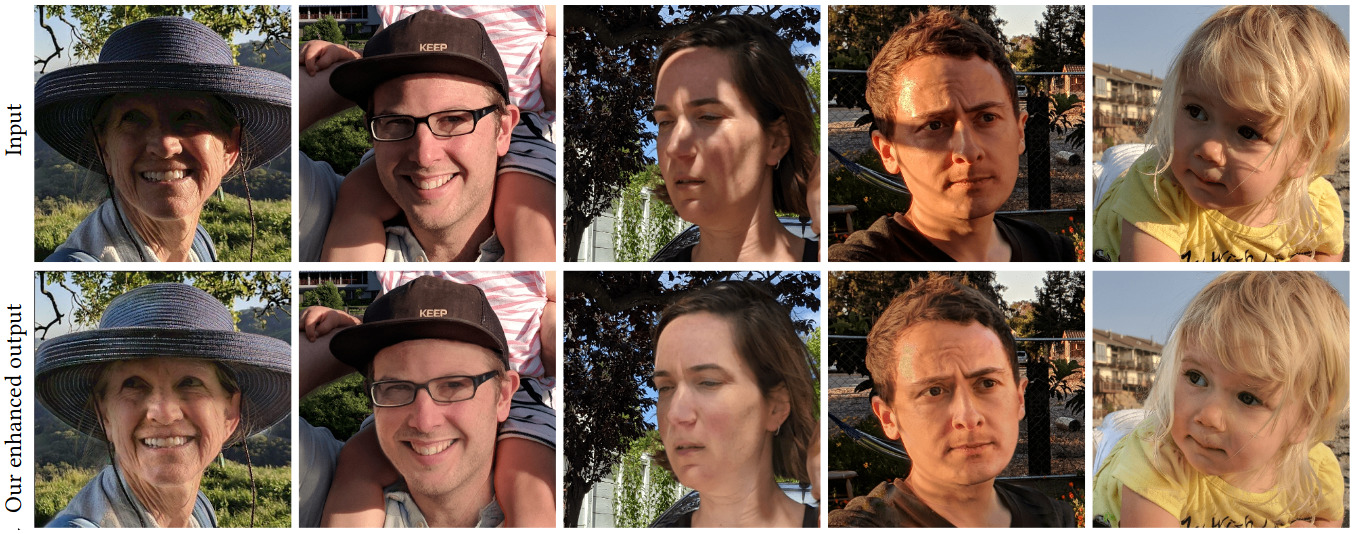
\includegraphics[width=0.7\linewidth]{img/biblio/shadow-removal}
        \caption{Suppression de l'ombre par apprentissage profond proposé par Zhang}
        \label{fig:03-shadow-removal}
    \end{figure}
    
    \subsection{Indices de télédétection}
    \label{sec:vegetation-indices}
    
    L'idée de base de l'imagerie hyperspectrale repose sur le fait que, pour tout matériau, la quantité de rayonnement réfléchi, absorbé ou émis dépend de la longueur d'onde. Donc la réponse spectrale du matériau varie selon un mode unique lié a sa composition moléculaire \cite{Mercan2011}. Cela signifie que, les signatures spectrales des matériaux, sont uniques et ces signatures peuvent être utilisées efficacement pour distinguer et identifier des surfaces (figure \ref{fig:03-surface-spectral-signature}).
    
    \begin{figure}[H]
        \centering
        %{\scriptsize (source: \cite{WANG2019154})} \\
        %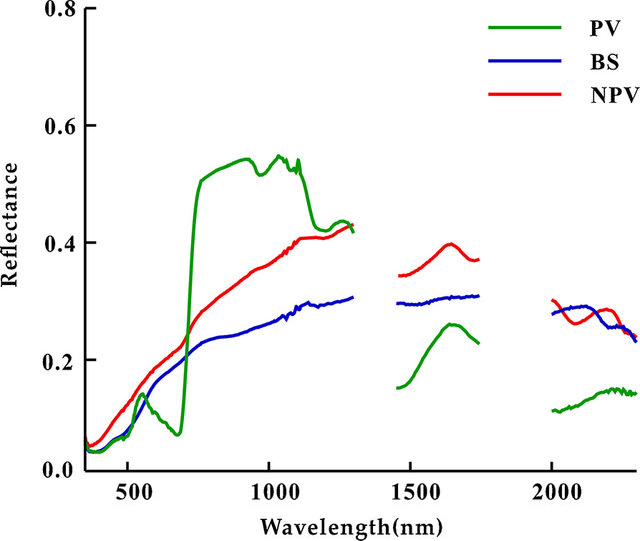
\includegraphics[height=8cm]{img/biblio/vegetation-spectral-signature} \\
        %{\scriptsize \textcolor{OliveGreen}{\large\textbullet} Végétation photosynthétique ; \textcolor{red}{\large\textbullet} Végétation non-photosynthétique ; \textcolor{blue}{\large\textbullet} Sol nu}
        %{\scriptsize (source: \cite{WANG2019154})} \\
        {\scriptsize (source: \cite{Mercan2011})} \\
        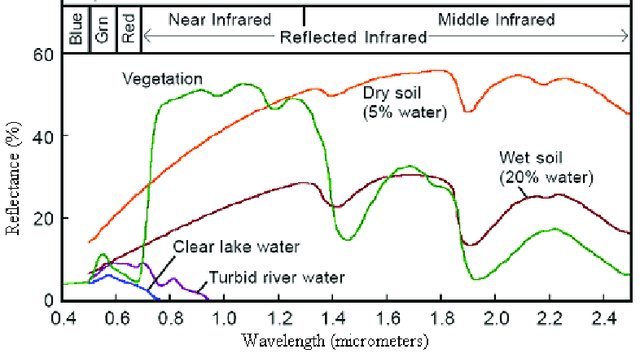
\includegraphics[height=5.5cm]{img/biblio/surface-spectral-signature} \\
        \caption{Signatures spectrales de certains matériaux}
        \label{fig:03-surface-spectral-signature}
    \end{figure}
    
    \subsubsection{Signature spectrale des plantes} 
    Les plantes se caractérisent, d'une part par leurs compositions moléculaires et d'autre part par leurs structures cellulaires. La figure \ref{fig:03-plant-cellular-structure} montre la structure cellulaire d'une feuille de dicotylédone (principal groupe des adventices). On y trouve deux épidermes (dessus/dessous) et entre ceux-ci se trouve la couche mésophylle \cite{ben2016utilisation}. La couche supérieure du mésophylle est composée de cellules contenant, entre autres, la chlorophylle (Chl a et Chl b) formées lors du processus de photosynthèse. Cette couche supérieure absorbe en grande partie le spectre visible, elle contient également d'autres pigments comme les carotènes, mais n'interfère pas avec d'autres longueurs d'onde. La couche inférieure, spongieuse, du mésophylle est constituée de cellules irrégulières et d'espaces vides qui eux réfléchissent de manière importante toutes les longueurs d'onde (diffère chez les monocotylédones).
    
    \begin{figure}[H]
        \centering
        {\scriptsize (source: \cite{ben2016utilisation})} \\
        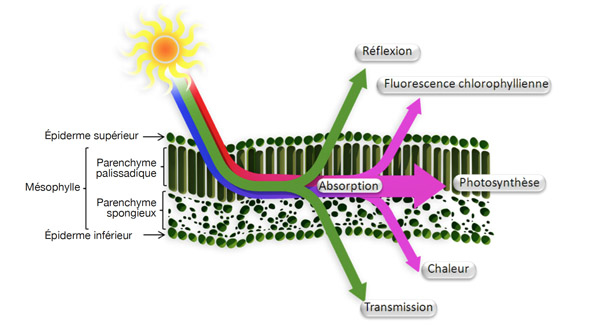
\includegraphics[width=0.6\linewidth]{img/biblio/plant-cellular-structure}
        \caption{Structure cellulaire d'une feuille et interaction avec le spectre électromagnétique}
        \label{fig:03-plant-cellular-structure}
    \end{figure}
    
    \par En conséquence, les plantes ont une faible réflectance pour les longueurs d'onde entre \SI{400}{nm} (bleu) et \SI{700}{nm} (rouge) avec un maximum autour de \SI{550}{nm} (vert). À contrario, les plantes ont une forte réflectance dans le proche infrarouge (entre \SI{850}{nm} et \SI{1300}{nm}). La région du red-edge, qui représente la zone de transition entre le rouge et le proche infrarouge (approximativement entre \SI{675}{nm} et \SI{750}{nm}), se caractérise par une brusque augmentation de la réflectance. La concentration en chlorophylle déplace la réflectance dans le red-edge. Une diminution de la concentration engendre une pente plus douce dans cette région. De la même façon, une diminution de la concentration d'eau change la couche inférieure, spongieuse, du mésophylle et donc la réflectance dans l'infrarouge. Finalement dans le domaine de l'infrarouge court (short wave infrared, SWIR), le spectre de réflectance présente trois pics d'absorption en \SI{1450}{nm}, \SI{1950}{nm} et \SI{2500}{nm} due à la présence d'eau dans les feuilles. L'ensemble de ces éléments sont visibles sur la courbe verte (végétation) de la figure \ref{fig:03-surface-spectral-signature}. 
    
    \subsubsection{Indices de végétation} Mesurer et interpréter le rayonnement électromagnétique permettent d'établir des indices qui caractérisent les surfaces observées. Ces indices évoluent en fonction de la nature de l'objet (sol, eau, végétation) et sont donc particulièrement utiles pour la segmentation. Il existe une base de données \url{indexdatabase.de} qui recense ces différents indices de télédétection. Pour chaque forme d'indice, leurs variantes (en fonction du matériel d'acquisition) sont également mises à disposition. Certains indices permettent par exemple d'estimer la composition des sols \cite{Dhawale2021}.
    
    \par Observer le spectre de réflectance des plantes a permis d'établir des indicateurs physiologiques, phénologiques et physiques. Le NDVI pour ``Normalized Difference Vegetation Index'' est probablement l'indice de végétation le plus populaire et repose sur les connaissances empiriques précédemment exposées. Le NDVI se calcule à partir de la réflectance obtenue pour deux bandes spectrales : $NDVI = (N-R) \div (N+R)$ avec $N$ le proche infrarouge ($\approx \SI{850}{nm}$) et $R$ le rouge ($\approx \SI{650}{nm}$). Les valeurs théoriques du NDVI sont comprises entre $-1$ et $1$, celles-ci sont bornées entre 0 et 1 dans le cas de la végétation. Pour la végétation, le NDVI renseigne sur l'état sanitaire d'un végétal. Une valeur de NDVI faible induit une faible activité photo-synthétique d'une plante et inversement. Il existe une grande variété d'indices de végétation, dont tous reposent sur des combinaisons de réflectance pour différents domaines spectraux. Les articles \cite{pmid29997682,XueJinru,Zhang2017ImagePT} mettent en exergue les indices ayant été testés pour détecter la présence de végétaux sur des images multispectrales. Ces indices reposent principalement sur une différence de réflectance entre le visible et le proche infrarouge. Ces indices n'utilisent pas plus de deux ou trois bandes spectrales ce qui diminue leurs potentiels de discrimination.
    
    \begin{figure}[H]
        \centering
        {\scriptsize (source: \url{earthdaily.com})} \\
        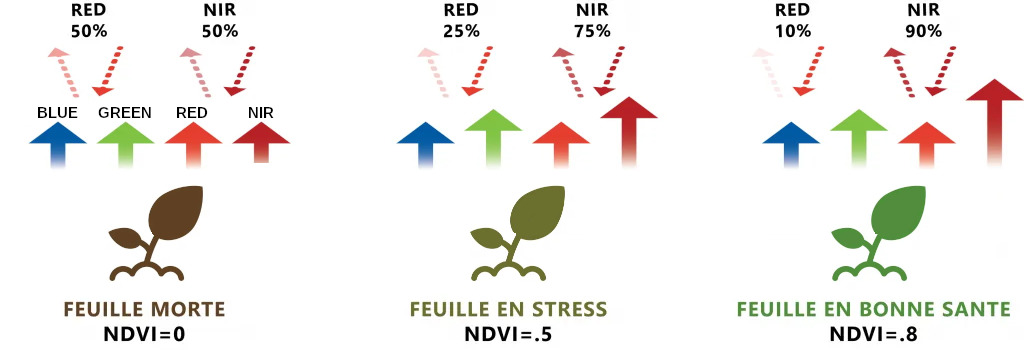
\includegraphics[width=0.7\linewidth]{img/biblio/base-ndvi-empiric}
        \caption{Une faible activité photo-synthétique induit une faible valeur de NDVI}
        \label{fig:03-base-ndvi-empiric}
    \end{figure}
    
    \newpage
    \subsubsection{Limite des indices de végétation} Bien que ces indices soient largement utilisés, ils ne permettent pas une utilisation optimale en conditions réelles. Leurs natures empiriques, l'influence de nombreux facteurs environnementaux, ainsi que le système d'acquisition sont des éléments qui jouent un rôle dans les performances de tels indices :
    \\
    \noindent
    \begin{itemize}
        \item \textbf{Bandes spectrales} Pour établir des indices de télédétection, on a recours à l'imagerie hyperspectrale. Selon la scène observée, le choix des ``meilleures'' bandes spectrales se fait à partir d'un échantillon d'acquisition. Elles seront ensuite sélectionnées pour être utilisées dans des capteurs multi-spectraux. Finalement, les indices sont eux même basés sur une ou deux bandes spectrales et diminuent encore le potentiel de discrimination.
        
        \item \textbf{Acquisition} Les conditions d'acquisition (jour, nuit, soleil, nuage, ombres, \dots) modifient la lumière incidente et donc les performances de ces indices \cite{Zhang2015}. Il y a également le mix spectral (mélange de signatures spectrales issues de différents matériaux) qui constitue une source d'erreur lorsque la résolution spatiale est insuffisante \cite{Louargant2017}, les petites adventices peuvent ne pas être détectées.
        
        \item \textbf{Calibration} Les indices de végétation reposent sur la réflectance. Une calibration doit être mise en œuvre et nécessite un dispositif d'étalonnage (section \ref{sec:correction-color} partie A). Cette calibration peut introduire des erreurs, puisque les résultats ne sont pas stables dans le temps (changement de luminosité au cours de la journée, passage d'un nuage, \dots). Et difficilement utilisable en proxi-détection et en temps réel.
        
        \item \textbf{Plante} Le groupe d'appartenance de la plante est une source d'erreur : la classe de la plante (monocotylédone, dicotylédone, hétérotrophes \footnote{Les végétaux hétérotrophes prélèvent leurs nutriments par symbiose, parasitisme ou prédation}, photoautotrophes \footnote{Caractérise les végétaux chlorophylliens, faisant intervenir la photosynthèse}) \cite{WANG2019154}, leurs états sanitaires \cite{gay2003elaboration, alnaser:tel-01914978, fournier:pastel-00794011} (chaleur, eau, azote, nitrate, phosphate, \dots, maladies, \dots) \cite{PIEDALLU20192874}, leurs stades de développement (croissance/sénescence) \cite{Palanisamy2019}, sont autant de facteurs qui peuvent modifier la valeur d'un indice de végétation comme le NDVI, si bien qu'une plante peut ne pas être détectée (faux négatif).
        
        \item \textbf{Sol} Des corps étrangers sur le sol peuvent être détectés (faux positifs). Par exemple, certaines moisissures et bactéries changent la couleur du sol, de même que la présence de métaux et la teneur en eau.
        
    \end{itemize}
    
    \vspace{1em}
    Ces éléments démontrent rapidement que la détection de la végétation n'est pas un problème trivial. Même si ces indices ont été largement utilisés, des études récentes soulignent le faible niveau de discrimination pour l'estimation de la surface foliaire \cite{su11030864, rs13132617} et donc leurs performances relatives pour une segmentation sol/végétation.
    
    %rs13132617 >> Moreover, if a VI was only sensitive to a limited number of factors, the confidence intervals of these factors might be large and overlapping, and, thus, the results were not robust.
    % https://www.researchgate.net/publication/233026449_A_new_vegetation_index_based_on_the_universal_pattern_decomposition_method >> image of spectral signature of yellow/green/dead leaf
    
    %La composition moléculaire des plantes peuvent fluctuer au cours de leurs vies, par exemple en cas de stresse environnemental, ces changements impacte alors la structure cellulaire \cite{} et peuvent à leurs tours modifié le processus de photosynthèse.
    
    %\begin{figure}[H]
    %	\centering
    %	{\scriptsize (source: \cite{Palanisamy2019})} \\
    %	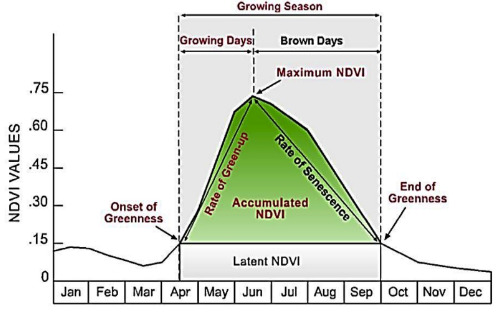
\includegraphics[width=0.5\linewidth]{img/biblio/ndvi-graph}
    %	\caption{Courbe NDVI hypothétique de réponse temporelle sur douze mois}
    %	\label{fig:03-ndvi-graph}
    %\end{figure}
    
    \newpage
    \section{Segmentation}
    \label{sec:segmentation}
    
    L'extraction d'informations à partir d'images s'effectue par le processus de segmentation. L'objectif de la procédure est d'extraire les composantes de l'image qui présentent un intérêt. La construction des régions d'intérêt est basée sur des caractéristiques de l'image telles que la couleur, la luminosité spectrale, la détection des contours, la similarité des pixels voisins ou la combinaison de ces propriétés, qui sont normalement intégrées à l'aide d'un processus d'apprentissage.
    
    \subsection{Segmentation sémantique}
    
    La segmentation sémantique consiste à classer les pixels selon leur classe d'appartenance. L'exemple le plus courant en agriculture de précision est la discrimination de la végétation (première classe) du reste (i.e. le sol, second classe). D'avantage de classes peuvent être définies. % Dans le cas de la segmentation sol/végétation, l'approche la plus largement utilisée consiste à calculer un indice de végétation sur lequel une technique de seuillage est appliquée.
    
    \paragraph{Thresolding} La méthode la plus simple consiste à déterminer un seuil entre les classes, à partir de l'indice de végétation pour l'exemple de la segmentation sol/végétation. Le seuil peut être fixé manuellement, ou par apprentissage. Les méthodes de seuillage peuvent aussi se reposer sur des algorithmes de classification. Cette approche est peu robuste aux changements d'illumination.
    
    \paragraph{Otsu} C'est une version améliorée du seuillage, consistant en une recherche automatique et exhaustive du seuil de segmentation. L'algorithme recherche le seuil qui minimise la variance intra-classe, définie comme une somme pondérée des variances de deux classes. La méthode montre de bonne performance si l'histogramme a une distribution bi-modale. Ceci est le cas pour un indice de végétation lorsque le sol est suffisamment visible sur l'image. À contrario, lorsque la végétation recouvre majoritairement le sol (ou lorsqu'elle est peu présente), la segmentation échoue. Cette méthode, non-supervisée, à l'avantage de bien gérer les gradients de luminosité contrairement à un seuillage simple. Cette approche est largement utilisée en agriculture \cite{Sa2017}, mais souffre de précision sur les cas limites, tels que les feuilles fines.
    
    \paragraph{Grabcut} L'algorithme apprend un modèle de mixture gaussienne pour classer l'information à partir de la zone d'intérêt et d'un masque. Ensuite, un graphe est construit à partir de la distribution des pixels entre foreground / background. Chaque pixel est connecté au nœud correspondant avec un poids d'appartenance en fonction de la probabilité de distribution de l'ensemble des pixels. Finalement, un algorithme de mincut est utilisé pour segmenter le graphe, donc l'image. Une application sur des données spectrales existe \cite{estrada2004spectral}.
    
    \begin{figure}[H]
        \centering
        \source{\cite{Gring2012SemanticSU}}
        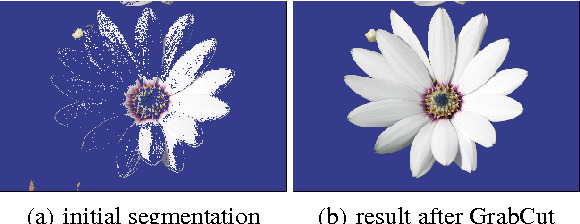
\includegraphics[width=0.55\linewidth]{img/biblio/segmentation-grabcut}
        \caption{Segmentation Grabcut}
        \label{fig:03-segmentation-grabcut}
    \end{figure}
    
    \newpage
    \paragraph{Chaîne de Markov} \cite{derrode2003segmentation} L'image est transformée en signal 1D par exemple avec un algorithme de \og Space-filling curve \fg comme Hilbert-Peano, Z-order, Sierpiński ou Moore, le graphe linéaire ainsi obtenu (chaîne) est stationnaire, ces probabilités sont déduites des probabilités conjointes qui sont indépendantes. La classe du premier pixel est tirée aléatoirement à partir de la distribution a posteriori. Par la suite, pour chaque nouveau pixel, la probabilité de transition est calculée, la classe du pixel précédent est fixée, et la classe du pixel suivant est obtenue par un prélèvement aléatoire selon cette distribution. La distribution a posteriori peut être estimée et initialisée grâce à l'histogramme de l'image et en utilisant l'algorithme des k-means (moyenne, déviation, écart-type).
    
    \paragraph{Champ de Markov} \cite{rechid2011segmentation} Le principe est similaire aux chaînes de Markov, le graphe de représentation est alors 2D et le nombre de transitions est plus important, ce qui augmente les temps de calcul. Une étude est présentée dans un contexte agronomique \cite{Yue2016}. En revanche, l'approche est largement utilisée en segmentation d'images médicales. L'étude de \cite{Salzenstein2006FuzzyMR} propose une comparaison entre les chaînes de Markov et les champs de Markov appliqués aux données multispectrales, les résultats montrent une meilleure homogénéité des régions segmentées par les champs de Markov, bien que statistiquement, les chaînes de Markov semblent donner de meilleurs résultats. Une application avancée permet de combiner les avantages de l'apprentissage profond et des champs de Markov cachés \cite{DBLP:journals/corr/LiuLLLT16}.
    
    %\begin{figure}[H]
    %	\centering
    %	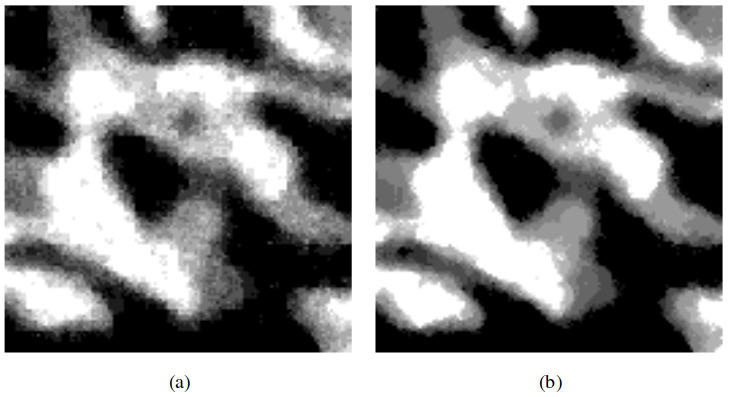
\includegraphics[width=0.3\linewidth]{img/biblio/segmentation-markov}
    %	\caption{(a) châine de markov, (b) champ de Markov \cite{Salzenstein2006FuzzyMR} }
    %	\label{fig:03-markov}
    %\end{figure}
    
    \paragraph{Apprentissage profond} Les réseaux de neurones convolutifs basés sur une structure d'encodeur-décodeur sont très populaires et ont démontrés leurs performances dans la discrimination des adventices \cite{brilhador2019classification, YOU2020105750, khan2020ced}. L'amont du réseau utilise une série de convolutions et de sous-échantillonnages (pooling), cet ensemble est généralement appelé encodeur et génère des informations sur l'objet, telles que sa forme et sa taille à une résolution inférieure. La sortie est ensuite sur-échantillonnée (upsampling) par interpolation bilinéaire ou par une série de convolutions transposées en aval du réseau, ensemble appelé décodeur. Il cherche à distribuer les informations basses résolutions de l'encodeur vers les informations de haute résolution pour obtenir une carte de segmentation dans la résolution initiale. Ces éléments sont présentés dans la figure \ref{fig:03-encoder-decoder}.
    
    \vfill
    \begin{figure}[H]
        \centering
        {\scriptsize (source: \cite{ma2019fully})}\\
        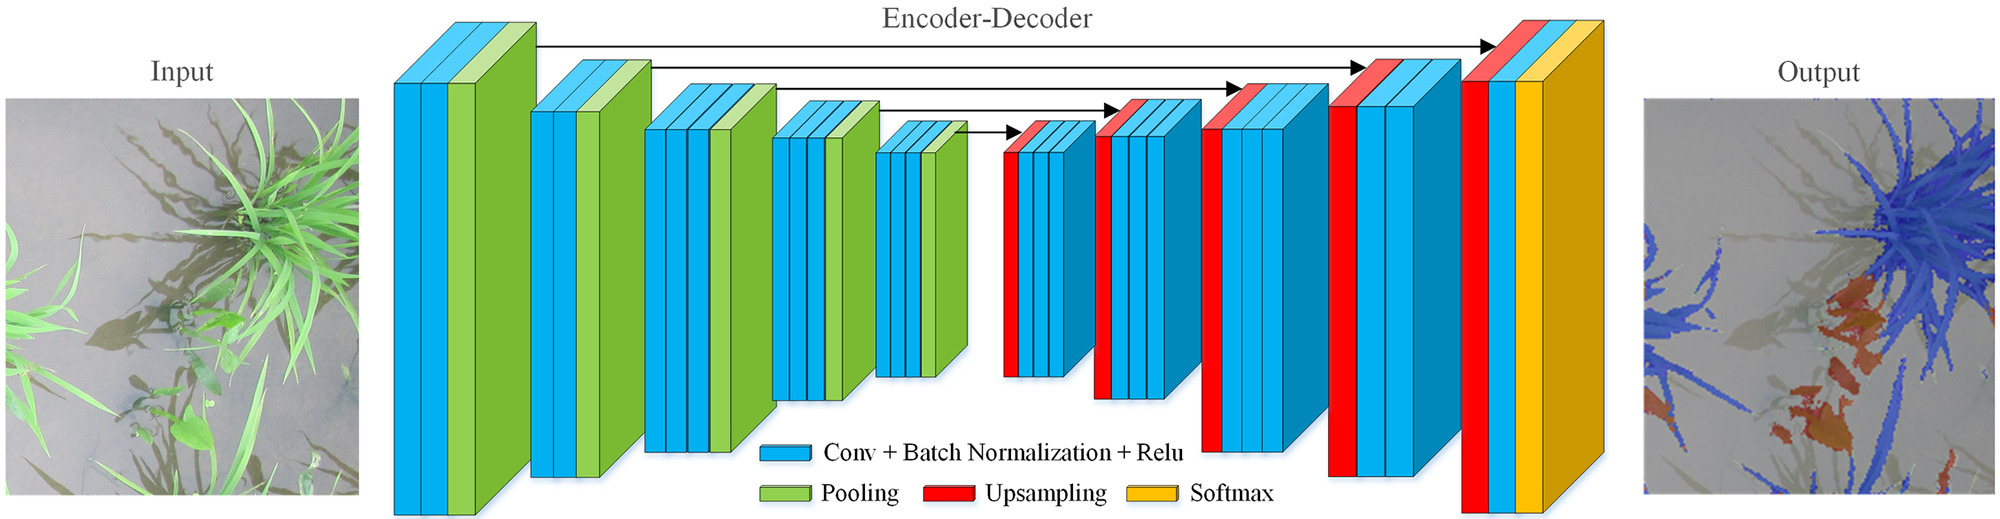
\includegraphics[width=\linewidth]{img/biblio/encoder-decoder}
        \caption{Architecture encodeur-décodeur d'un réseau convolutif}
        \label{fig:03-encoder-decoder}
    \end{figure}
    \vfill
    
    % Au niveau inférieur, les neurones contiennes des informations sur une petite zone de l'image, tandis qu'au niveau supérieur, le neurone contient des informations sur une grande zone de l'image. Par conséquent, à mesure que nous ajoutons des couches, la taille de l'image diminue, tandis que le nombre de canaux augmente. Lorsque nous augmentons la résolution, nous réduisons le nombre de canaux car nous renvoyons des informations de bas niveau. C'est ce qu'on appelle la structure encodeur-décodeur
    
    %Si nous empilons simplement les couches de l'encodeur et du décodeur, des informations de bas niveau peuvent être perdues. Par conséquent, les limites de la carte de segmentation générée par le décodeur peuvent être inexactes. Pour compenser les informations manquantes, nous laissons le décodeur accéder aux caractéristiques de bas niveau générées par la couche d'encodage. Ceci est fait en sautant la connexion. La sortie intermédiaire de l'encodeur est ajoutée/connectée à l'entrée de la couche intermédiaire du décodeur à une position appropriée. La connexion sautée de la couche précédente fournit à la couche du décodeur les informations nécessaires pour créer une frontière précise.
    
    \newpage
    \subsection{Segmentation en région} 
    
    Au lieu de ne travailler qu'avec des pixels (segmentation sémantique), on découpe l'image en région. L'utilisation de régions présente deux avantages majeurs (i) calculer des caractéristiques sur des régions plus significatives et (ii) réduire les entités en entrée pour les étapes suivantes.
    
    \paragraph{Découpage régulier} L'image est simplement découpée en sous-images de tailles fixes (avec ou sans recouvrement figure \ref{fig:03-patch-segmentation}). La taille a un impact important : trop petite, elle manquera d'information discriminante et trop grande, elle pourra contenir des mélanges des classes (culture, adventice, sol) rendant la classification difficile. La discrimination des adventices se résume alors à un problème de classification de texture. Des approches multi-échelles sont aussi possibles \cite{HU2020105520} mais ne permettent pas de détecter les plus petites adventices.	
    
    \begin{figure}[H]
        \centering
        {\scriptsize (source: \cite{brilhador2019classification})} \\
        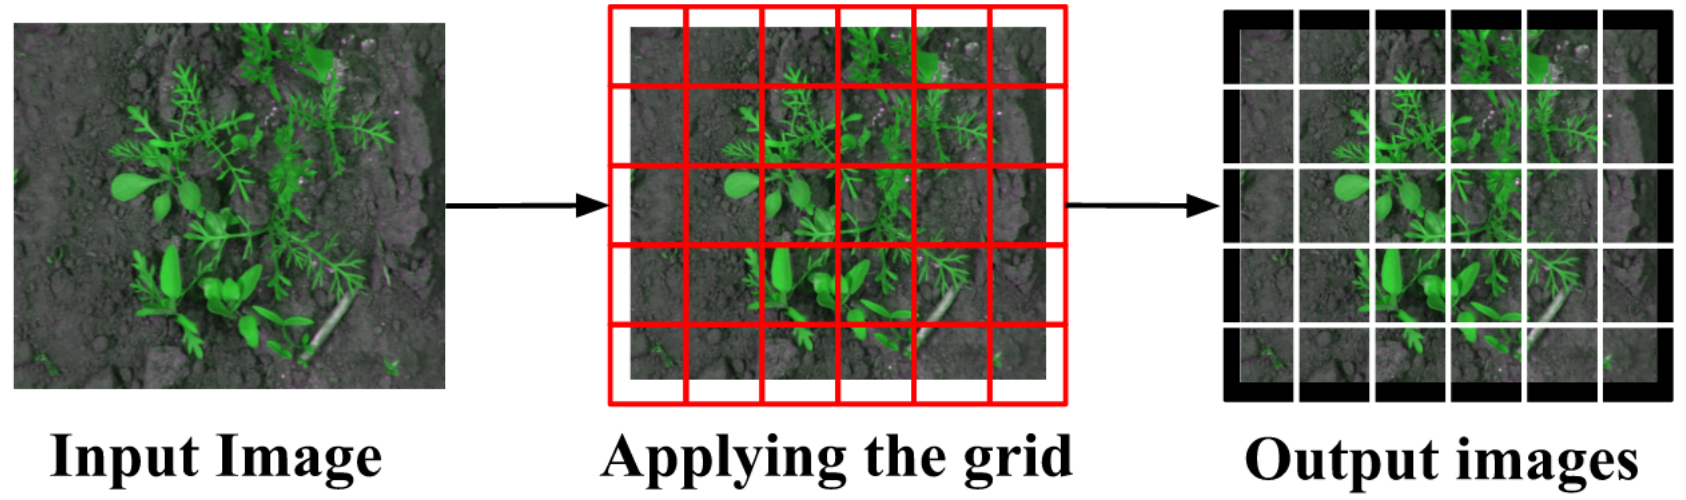
\includegraphics[width=0.7\linewidth]{img/biblio/patch-segmentation}
        \caption{Découpage régulier sans recouvrement}
        \label{fig:03-patch-segmentation}
    \end{figure}
    
    
    \paragraph{Composantes connexes} On peut récupérer les zones distinctes dans l'image à l'aide d'un algorithme, après une première segmentation sémantique (par exemple sol/végétation). Dans le cas de la discrimination des adventices, cette approche ne permet pas de distinguer les feuilles, des plantes, des groupes de plantes. Une composante connexe peut donc être composée de cultures et d'adventices en proportions variables, en fonction du taux de couverture végétale. Extraire des propriétés sur ces zones et essayer de les discriminer est donc peu fiables \cite{rs10050761}.
    
    \paragraph{Template matching} C'est une méthode permettant de rechercher et de trouver l'emplacement d'une image modèle dans une image plus grande. Il suffit de faire glisser l'image modèle sur l'image d'entrée et de comparer le modèle et avec la portion de l'image d'entrée. Cette approche est peu robuste pour de la détection de plante ou de feuille, car ces dernières ont une grande variabilité. De plus, c'est une méthode lourde en temps de calcul bien qu'elle ait été utilisée pour la détection des bananiers \cite{ZHOU201458}.
    
    \paragraph{Transformation de Hough} Il existe deux grandes variantes de la transformée de Hough qui permettent de détecter des formes fixes dans l'image, par exemple des lignes ou des ellipses. Ainsi cette transformée a été utilisée pour détecter les rangs de culture. Les composantes connexes entre les lignes de culture sont principalement des adventices \cite{rs10050761}. La détection des ellipses par transformée de Hough présente aussi des avantages : les formes des feuilles des dicotylédones étant souvent proches d'une ellipse cette transformée permet de les détecter \cite{Kumar2018, zhonghua2020automatic}. Des techniques similaires peuvent également détecter les ``blobs'' (Laplacian of Gaussian, Difference of Gaussian, Determinant of Hessian, Maximally stable extremal region, \dots).
    
    \newpage
    \paragraph{Super-pixel} Un super-pixel est un groupe de pixels connectés avec des couleurs ou des niveaux de gris similaires. La segmentation des super-pixels consiste donc, à diviser une image en centaines de super-pixels ne se chevauchant pas. Cette approche a été testée dans le domaine de l'agriculture de précision avec une approche multi-échelle \cite{DBLP:journals/corr/abs-1805-12395} proposant des résultats de classification intéressants $\sim \SI{90}{\percent}$. Cette approche, pertinente à haute altitude présente des défauts majeurs en proxi-détection avec un paramètre difficile à déterminer : la taille des super-pixels. Les adventices et les cultures présentent des différences de taille notables (stade de développement) et de texture significatives. Ce qui donne des résultats instables en proxi-détection \cite{li2021identification}.
    
    \begin{figure}[H]
        \centering
        {\scriptsize (source: \cite{DBLP:journals/corr/abs-1805-12395})} \\
        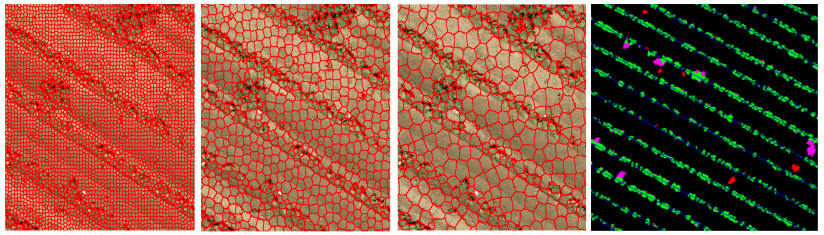
\includegraphics[width=0.7\linewidth]{img/biblio/segmentation-superpixel}
        \caption{Analyse multi-échelle des super-pixels et classification}
        \label{fig:03-superpixel}
    \end{figure}
    
    %Ce type d'approche nécessite une initialisation, par exemple les maximums locaux d'un indice de végétation ou d'autres propriétés telles-que Harris, SIFT, SURF, ORB, \dots.  Le mécanisme s'adresse à la segmentation Foreground / Background (sol/végétation dans notre cas). Il prend en entrée une région de l'image contenant intégralement l'objet à segmenter, ainsi qu'un masque représentant les zones à rejeter/inclure.
    
    \paragraph{Watershed} L'algorithme calcule les distances entre les bords des régions segmentées et les différents centres initialisés. Ensuite, l'algorithme distingue autant de sous-régions qu'il y a de points culminants, et alimente chacune d'entre elles par l'incrémentation des pixels voisins selon une propagation circulaire de proche en proche. Les régions sont isolées lorsqu'un même ensemble de pixels est candidat pour intégrer deux régions différentes.
    
    \begin{figure}[H]
        \centering
        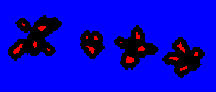
\includegraphics[width=0.25\textwidth]{img/biblio/segmentation-watershed-init}
        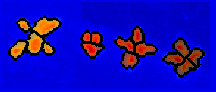
\includegraphics[width=0.25\textwidth]{img/biblio/segmentation-watershed} \\
        {\scriptsize les zones d'initialisation à gauche et à droite, en couleur les régions étendues}
        \caption{Exemple de watershed sur des images drones}
        \label{fig:03-watershed-region}
    \end{figure}
    
    Ce type d'approche est donc très utile pour agrandir la segmentation, en particulier, on peut déterminer facilement le sol grâce à la méthode de seuillage de Otsu et les feuilles via des descripteurs de texture. L'algorithme Watershed propose alors une division interne des plantes (figure \ref{fig:03-watershed-region}). Mais le choix des centres reste difficile à déterminer, rendant l'initialisation de ces derniers très dépendants de la résolution spatiale. Ainsi des approches complémentaires sont souvent nécessaires.
    
    %\paragraph{Distance Regularized Level-set} La méthode level-set est bien connue pour l'extraction du contour et la segmentation de l'objet.
    
    \paragraph{Chan-vese}
    Le modèle proposé par Chan et Vese, est l'un des modèles les plus populaires pour la segmentation des images en région. Il combine le modèle Mumford-Shah simplifié et la méthode LevelSet pour résoudre un problème de minimisation de l'énergie. Le modèle est largement appliqué aux images qui doivent être segmentées en deux régions : cible et arrière-plan. Ce type de segmentation a été utilisé avec succès pour la segmentation de feuilles qui se chevauchent en champ proche \cite{WANG20181}. Bien que l'approche donne des résultats intéressants dans la littérature, le temps de calcul est important, ce qui est également à prendre en considération.
    
    \paragraph{Active contours} Le modèle de contour actif est une méthode d'ajustement d'une courbe aux lignes ou aux bords d'un objet dans une image. L'algorithme fonctionne en minimisant l'énergie définie en partie par l'image (texture, gradient) et en partie par la forme de la courbe (courbure). En ce sens, l'algorithme est similaire aux super-pixels. Les contours actifs sont utilisés pour identifier les plantes par leurs fleurs \cite{MANH2001139, flower2012}. Une amélioration pour reconnaître les arbres par leurs feuilles a été proposée par \cite{Cerutti2011}, une contrainte est ajoutée aux contours actifs en utilisant un modèle de feuille polygonale. Cette amélioration suppose une connaissance à priori de la forme dans la scène qui doit être ``complète''.
    
    \begin{figure}[H]
        \centering
        {\scriptsize (source: \cite{Cerutti2011})} \\
        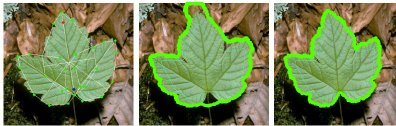
\includegraphics[width=0.7\linewidth]{img/biblio/segmentation-active-contour}
        \caption{Polygone initial, contour actif, et contour avec contrainte}
        \label{fig:03-segmentation-active-contour}
    \end{figure}
    
    % \paragraph{Détection des blobs} Principe similaire à la transformation de Hough, mais basé sur une analyse des gradients dans l'image.
    
    \paragraph{Apprentissage profond} Récemment, des améliorations considérables en matière de détection d'objets ont été obtenues grâce aux réseaux de neurones convolutifs. Le même principe que pour la segmentation sémantique est utilisé. Cependant la partie ``décodeur'' est remplacée par un réseau de prédiction des boîtes englobantes (bounding-box en anglais). Le réseau proposera par exemple une sortie de taille $(4+2) \times 1000$, soit 1000 objets à détecter avec leurs positions $[x,y,width,height]$ ainsi que la classe et le score de confiance en cette prédiction $[class,score]$. Finalement, seules les boîtes englobantes avec un score suffisant sont retenues.
    
    \begin{figure}[H]
        \centering
        {\scriptsize (source: \cite{app10020612})} \\
        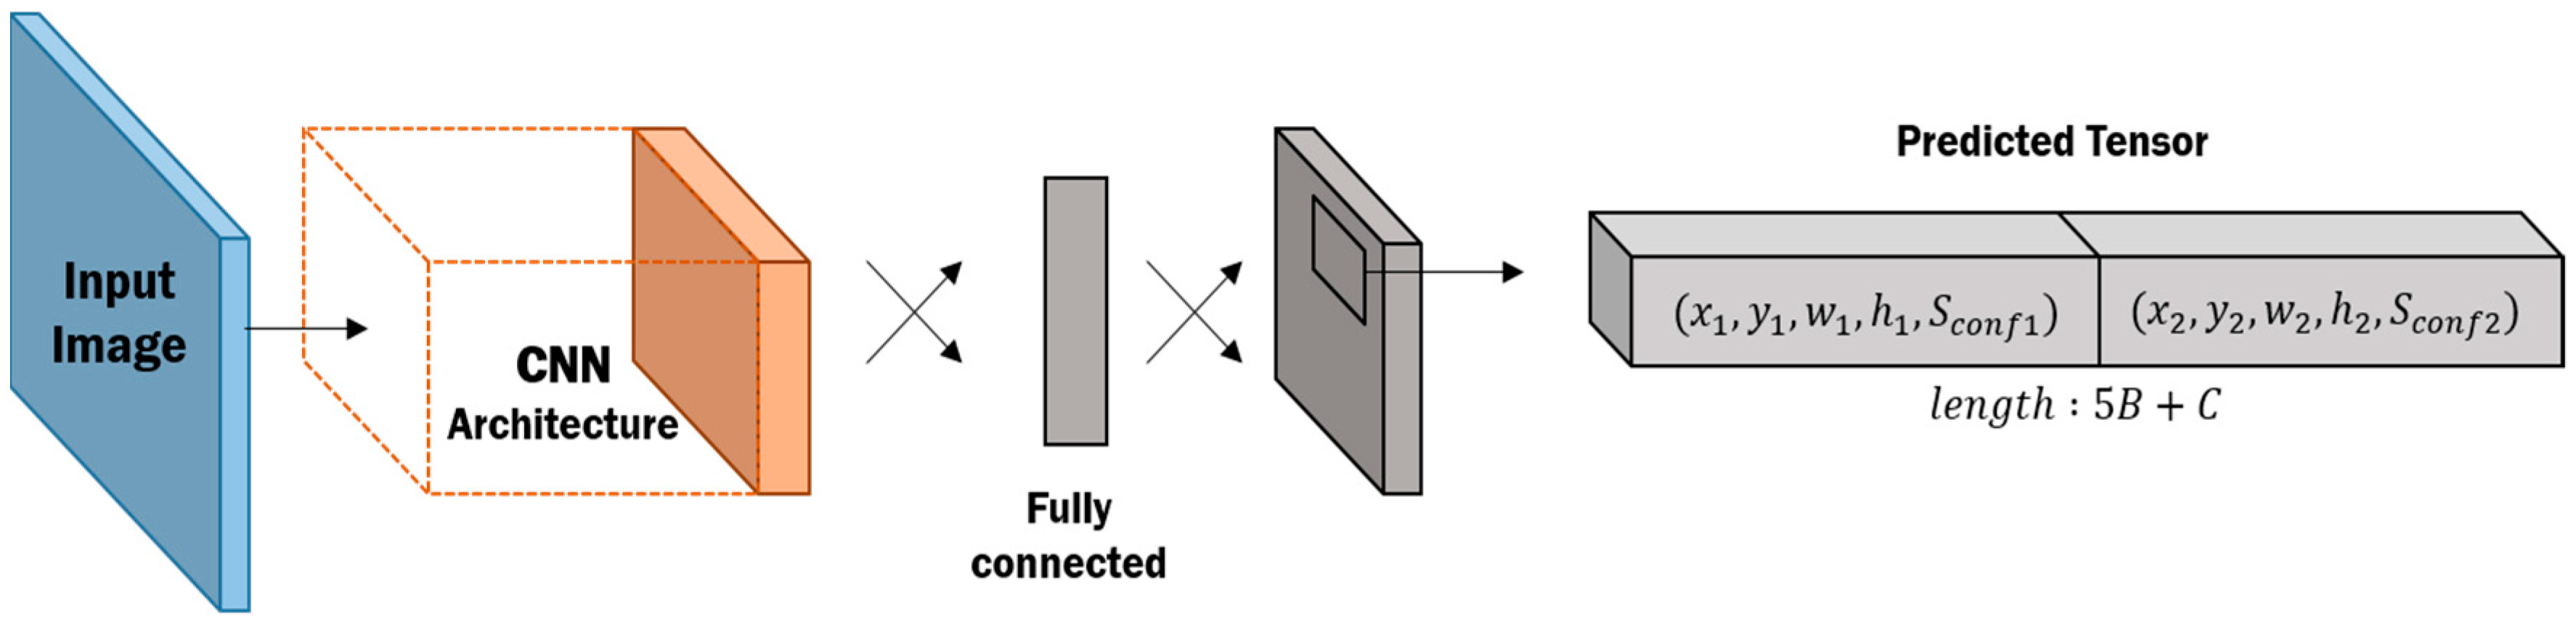
\includegraphics[width=\linewidth]{img/biblio/segmentation-object}
        \caption{Structure d'un réseau ``You Only Look Once'' (YOLO)}
        \label{fig:03-segmentation-object}
    \end{figure}
    
    Ce type d'approche détecte généralement plusieurs fois le même objet avec un décalage, pour pallier cet effet un algorithme de non-max suppression (NMS) est alors utilisé pour combiner les boites qui se superposent. Ce dernier point est problématique, car plus la densité d'objets est forte, plus il y aura des fusions et donc des non-détections. L'utilisation des CNN et plus particulièrement l'architecture YOLO (You Only Look Once) a été utilisée pour la discrimination des adventices \cite{rs13122288} mais n'est donc pas envisageable pour les stades de développement précoces et avancés. En agriculture de précision la revue \cite{s19051058} définit un ensemble de jeux de données (cultures, adventices, fruits, \dots) et leurs évaluations à travers différents modèles de détection, dont le modèle YOLO.
    
    \newpage
    \subsection{Segmentation des instances}
    
    La segmentation des instances consiste à la fois à détecter les objets et leurs masques de segmentation individuelle. Ici, seule l'utilisation des réseaux de neurones donne des résultats prometteurs. Il existe plusieurs variantes \cite{Hafiz_2020} à cette démarche, dont :
    
    \paragraph{Détection puis segmentation} La première consiste à utiliser une segmentation des objets, puis pour chaque objet détecté une segmentation sémantique est utilisée pour prédire le masque de segmentation de chaque objet. Ce type de méthode nécessite une base d'apprentissage importante. La détection d'objet peut être difficile sur les petits objets, comme nous l'avons vu précédemment, repose sur l'algorithme NMS (non-max suppresion) qui occasionne des mauvaises détections en scène dense. Puis le masque est prédit avec un second réseau, dont la taille de sortie est petite et fixe, l'ajustement du masque vers l'objet détecté se fait par étirement ce qui explique la qualité des masques générés (figure \ref{fig:03-segmentation-mask-rcnn}).
    
    \begin{figure}[H]
        \centering
        {\scriptsize (source: \cite{Jung2019})} \\
        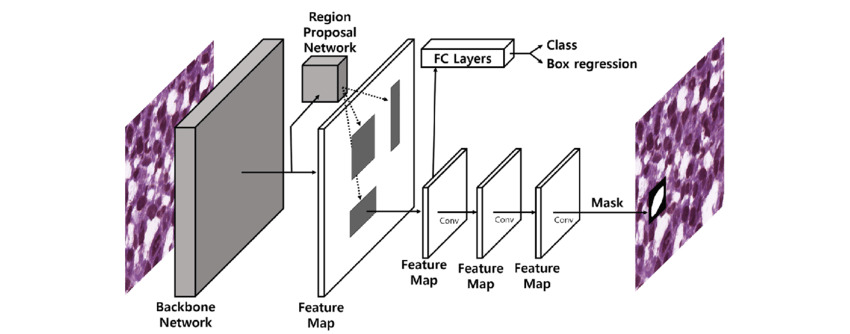
\includegraphics[width=\linewidth]{img/biblio/segmentation-mask-rcnn}
        \caption{Architecture d'un réseau de type Mask-RCNN}
        \label{fig:03-segmentation-mask-rcnn}
    \end{figure}
    
    Cette approche est utilisée par le consortium WeedElec \cite{champ:hal-02910844} dans le challenge RoSE, à travers une architecture mask-rcnn (figure \ref{fig:03-segmentation-mask-rcnn}), les ``petites'' adventices ($<\SI{3.5}{\cm^2}$) sont détectées avec une précision moyenne de $\approx \SI{2}{\percent}$, les adventices émergentes sont donc inexistantes. Les adventices ``moyennes'' comprises entre $3.5$ et $\SI{9.5}{\cm^2}$ sont détectées à hauteur de $\approx \SI{35}{\percent}$ tandis que les plus grandes sont mieux détectées $\approx \SI{51}{\percent}$.
    
    \newpage
    \paragraph{Instance embedding} La technique consiste à apprendre une transformation de l'image vers un espace latent. Les pixels qui font partie de la même instance doivent être proches les uns des autres pour former un cluster, tandis qui les pixels des autres instances doivent s'éloigner. Cet espace latent est en fait une projection des propriétés des pixels avec leurs instances associées spatialement. Cette approche repose essentiellement sur un réseau de segmentation sémantique, cherchant à minimiser la variance spatiale des pixels des instances (composantes connexes) tout en maximisant la distance des clusters au sein de l'espace latent \ref{fig:03-segmentation-embeding}). Cette approche a été testée pour la segmentation de feuilles \cite{DBLP:journals/corr/abs-1708-02551, wu2020improving}. Mais du fait de cet espace latent, la présence d'ombre ou de réflexion spéculaire peuvent être sources d'erreurs.
    
    \begin{figure}[H]
        \centering
        {\scriptsize (source: \cite{DBLP:journals/corr/abs-1708-02551})} \\
        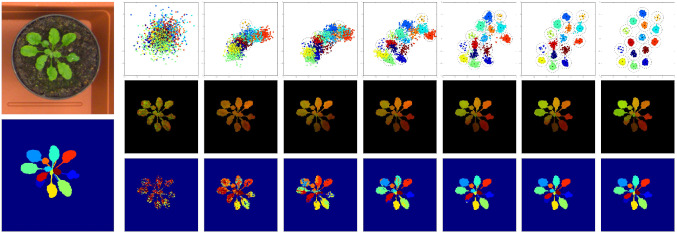
\includegraphics[width=\linewidth]{img/biblio/segmentation-embeding} \\
        \scriptsize À gauche : Image initial et vérité terrain. La rangée du milieu montre la sortie brute du réseau. La rangée supérieure montre l'espace latent avec les couleurs de chaques instances. La dernière rangée montre le résultat de la mise en cluster des embeddings par seuillage autour de leur centre de cluster. Chaque colonne montre l'apprentissage de l'espace latent.
        \caption{Espace latent et instances associées aux clusters}
        \label{fig:03-segmentation-embeding}
    \end{figure}
    
    \paragraph{Pixelwise instance} La segmentation sémantique peut être utilisée pour détecter des instances d'une autre manière, on parle alors de ``pixelwise instance segmentation''. L'idée repose essentiellement sur la détection des contours, donc la manipulation des classes de sortie (figure \ref{fig:03-segmentation-dcan}). Si cette approche n'est pas possible pour la détection des plantes, elle apporte néanmoins des possibilités pour la détection des feuilles \cite{morris2018pyramid} et des nucléus \cite{DBLP:journals/corr/abs-1810-06933}. La définition est simple et des fonctions de pertes avancées peuvent être mises en place afin d'en améliorer les performances.
    
    \begin{figure}[H]
        \centering
        {\scriptsize (source: \cite{DBLP:journals/corr/abs-1810-06933})} \\
        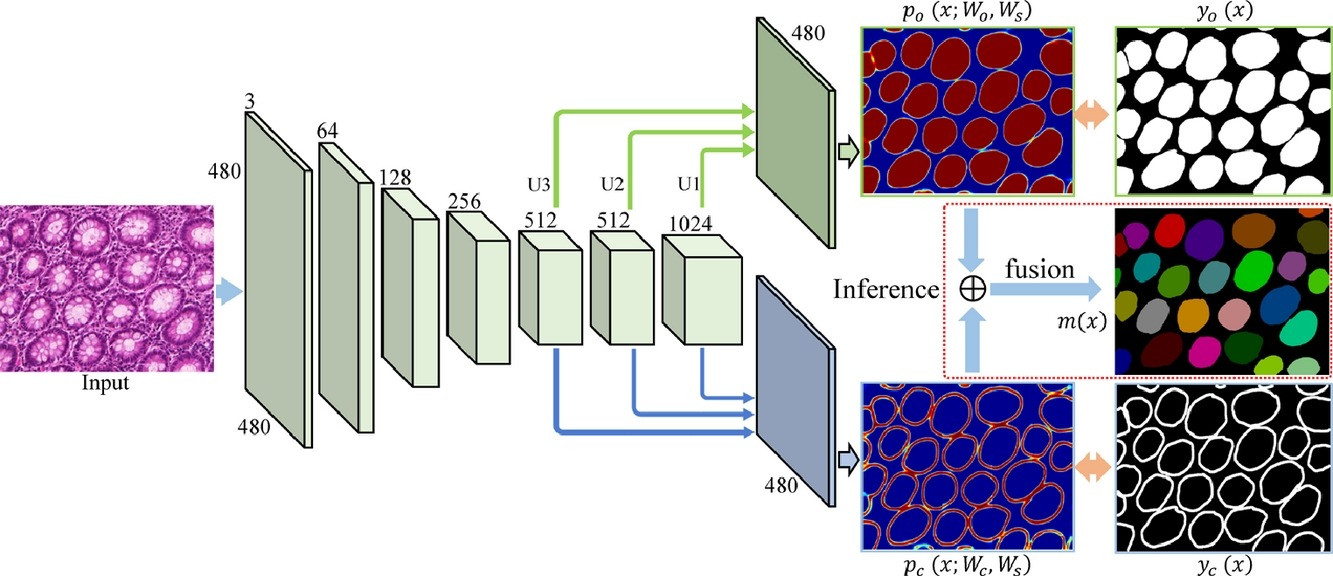
\includegraphics[width=0.7\linewidth]{img/biblio/segmentation-dcan}
        \caption{Segmentation des instances par détection des contours des nucléus}
        \label{fig:03-segmentation-dcan}
    \end{figure}
    
    %L'article suivant \url{https://www.jeremyjordan.me/semantic-segmentation/} explique en détail les différentes méthodes.
    
    \newpage
    \section{Extraction de propriétés}
    \label{sec:03-feature-extraction}
    
    % \cite{Liu2020}
    L'objectif de l'extraction de propriétés est de caractériser les éléments distincts qui ont été détectés par la phase de segmentation, avec des propriétés discriminantes. Pour chaque individu, un ensemble de caractéristiques est extrait et placé dans un ``vecteur de caractéristiques'' qui synthétise l'objet. Associé à une méthode de classification, le vecteur est utilisé pour classer l'objet dans une catégorie (sol, culture, adventice). L'extraction repose sur des informations différentes, visibles sur la figure \ref{fig:03-feature-extraction-flavor}.
    
    \begin{figure}[H]
        \centering
        %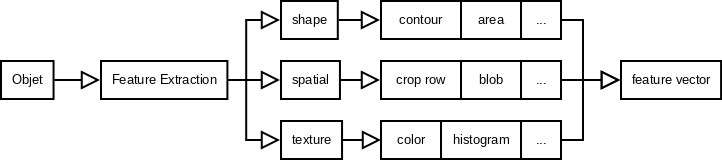
\includegraphics[height=3cm]{img/biblio/feature-extraction-flavor}
        \tikzset{
	ppblock/.style={
		rectangle,
		minimum size=6mm,
		very thick,
		draw=black!50,
		text centered,
		font=\ttfamily,
		minimum width=8em,
		minimum height=6mm,
		top color=white,
	},
	%
	figure/.style={
		rectangle,
		rectangle split,
		rectangle split parts=2,
		very thick,
		draw=black!50,
		text centered,
		append after command={
			\pgfextra
			\fill[top color=#1, bottom color=#1]
			(\tikzlastnode.one west) 
			[rounded corners] |- (\tikzlastnode.north) -| (\tikzlastnode.one east) 
			[sharp corners]   |- (\tikzlastnode.one split) -| cycle;
			\fill[top color=white, bottom color=#1]
			(\tikzlastnode.two west) 
			[rounded corners] |- (\tikzlastnode.south) -| (\tikzlastnode.two east)  
			[sharp corners]   |- (\tikzlastnode.one split) -| cycle;
			\endpgfextra
		},
	},
    splitted/.style={
        rectangle,
        rectangle split,
        rectangle split horizontal,
        rectangle split parts=2,
        very thick,
        draw=black!50,
        text centered,
        append after command={
            \pgfextra
            \fill[top color=white, bottom color=#1]
            (\tikzlastnode.south)
            [rounded corners] -| (\tikzlastnode.west) |- (\tikzlastnode.one north)
            [sharp corners]   -| (\tikzlastnode.one split) |- cycle;
            \fill[top color=white, bottom color=#1]
            (\tikzlastnode.two south)
            [rounded corners] -| (\tikzlastnode.east) |- (\tikzlastnode.north)
            [sharp corners]   -| (\tikzlastnode.one split) |- cycle;
            \endpgfextra
        },
    },
	%
	static/.style={ppblock, bottom color={black!20}},
	nonterminal/.style={ppblock, bottom color={blue!30}},
	terminal/.style={ppblock, bottom color={green!20}},
	algorithm/.style={ppblock, bottom color={yellow!50}},
	error/.style={ppblock, bottom color={red!20}},
	type/.style={ppblock, bottom color={red!20}},
	loss/.style={ppblock, dashed, bottom color={black!20}, font=\itshape},
	%
	tiny/.style={
		rounded rectangle,
		very thick,
		draw=black!50,
		top color=white,
		bottom color=red!20,
        text centered,
		font=\ttfamily,
	},
    operator/.style = {
        circle,
        scale=0.6,
        draw=black!50,
        top color=white,
        bottom color=red!20,
        font=\boldmath,
    },
	%
	skip loop/.style={to path={-- ++(0,#1) -| (\tikztotarget)}}
}

\begin{tikzpicture}[
        >=stealth',thick,
        tip/.style={->,shorten >=0.007pt},
        every node/.style={scale=0.7},
    ]
    \matrix[column sep=8mm, row sep=0mm, align=center] {
    	& & 
    	\node (shape) [type]   {Shape};         &
    	\node (contour) [nonterminal, minimum width=5em]   {Contour};
    	\node (area) [nonterminal, minimum width=5em,right of=contour, xshift=2.5em]   {Area};         
    	\node (p1) [tiny,right of=area, xshift=0.5em]   {\dots};         \\
    	%%%%%%%%%%%%%%%%%%%%%%%%
    	\node (obj)     [terminal]      {Object};         &
    	\node (fve)     [nonterminal]   {Feature\\Extraction};         &
    	\node (spatial) [type]   {Spatial};         &
    	\node (row)     [nonterminal, minimum width=5em]   {Crop row};         
    	\node (p2)      [tiny,right of=row, xshift=0.5em]   {\dots};         &
    	\node (ofv)     [terminal]      {Feature\\Vector};         \\
    	%%%%%%%%%%%%%%%%%%%%%%%%
    	& & 
    	\node (texture) [type]   {Texture};         &
    	\node (color) [nonterminal, minimum width=5em]   {Color};         
    	\node (hist) [nonterminal,right of=color, xshift=2.5em, minimum width=5em]   {Gradient};         
    	\node (p3) [tiny,right of=hist, xshift=0.5em]   {\dots};         \\
    };
    
	\begin{scope}
    	\draw[->]     (obj) to (fve);
    	\draw[->]     (fve.east) to [in=180, out=0, looseness=2] (shape.west);
    	\draw[->]     (fve.east) to [in=180, out=0, looseness=2] (spatial.west);
    	\draw[->]     (fve.east) to [in=180, out=0, looseness=2] (texture.west);
    	\draw[->]     (shape.east)   to [in=180, out=0] (contour.west);
    	\draw[->]     (spatial.east) to [in=180, out=0] (row.west);
    	\draw[->]     (texture.east) to [in=180, out=0] (color.west);
    	
    	\draw[->]     (p1.east) to [in=180, out=0, looseness=2] (ofv.west);
    	\draw[->]     (p2.east) to [in=180, out=0, looseness=2] (ofv.west);
    	\draw[->]     (p3.east) to [in=180, out=0, looseness=2] (ofv.west);
	\end{scope}
    
\end{tikzpicture}
        \caption{Types de caractéristiques}
        \label{fig:03-feature-extraction-flavor}
    \end{figure}
    
    On distingue les propriétés basées sur la géométrie (shape), celles qui se basent sur la texture et celles qui reposent sur une analyse spatiale des objets. Cette nomenclature n'est pas fixe, certaines études distinguent les propriétés de couleur, des propriétés spectrales au sein des propriétés de texture. Il existe bon nombre d'autres domaines où ces propriétés sont utilisées (granulométrie, médecine, \dots). Quelques exemples de propriété de chaque type sont présentés ci-après.
    
    \subsection{Propriétés géométriques} Les propriétés géométriques se basent sur différentes représentations du contour ou de l'intérieur de la forme. On y retrouve par exemple, le périmètre, l'aire de la surface convexe ou encore l'aire de la forme. La figure \ref{fig:03-feature-shape-leaf} montre un petit ensemble de propriétés de forme appliqué à une feuille. Ces propriétés, proposées par \cite{Gao2013ResearchOW} ont été utilisées pour la discrimination culture/adventices, les résultats de l'étude montre un taux de classification compris entre \SI{87.5}{\percent} et \SI{92.5}{\percent} sur les stades précoces et dans une parcelle peu infestée. Ces propriétés de forme sont invariantes par rotation, translation et changement de couleur. Mais elles sont néanmoins dépendantes de la résolution spatiale et fortement influencées par l'occultation et les performances de la segmentation.
    
    \begin{figure}[H]
        \centering
        \source{\cite{Gao2013ResearchOW}}
        % https://www.semanticscholar.org/paper/Research-of-Weeds-Classification-System-Based-on-Gao-Li/a067892ccbebefd602188edff93d14cc3ec847a1#extracted
        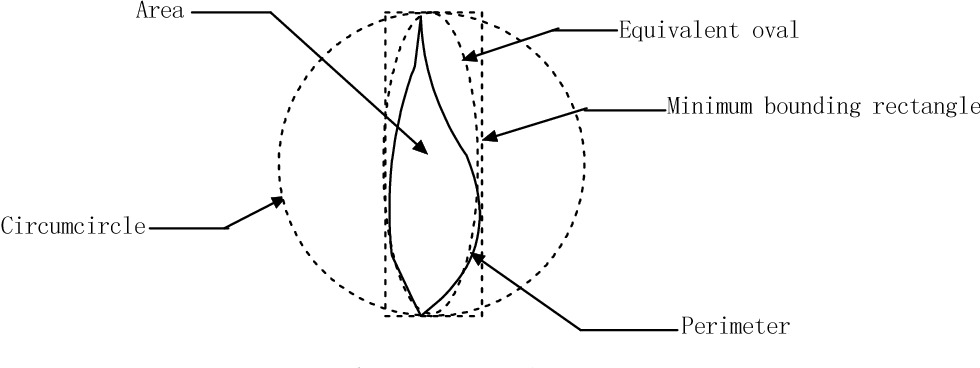
\includegraphics[width=0.7\linewidth]{img/biblio/feature-shape-leaf}
        \caption{Caractéristiques de la forme d'une feuille }
        \label{fig:03-feature-shape-leaf}
    \end{figure}
    
    \newpage
    \subsection{Propriétés spatiales} Les propriétés spatiales, se basent sur la détection d'éléments spécifiques de la scène. Le rang de culture est l'élément le plus remarquable en culture sarclée, cette connaissance a priori peut être utilisée pour discriminer les adventices situées dans l'inter-rang. On calcule alors la distance entre l'individu et son rang le plus proche, cette valeur caractérise l'objet (Figure \ref{fig:03-feature-crop-row}). Cette seule propriété est insuffisante pour caractériser et discriminer les adventices intra-rang. Le rang peut être défini automatiquement en plaçant des points GPS/GNSS durant le semis \cite{Griepentrog2005} ou par détection sur l'image \cite{MRNL2016}. Lorsque le taux d'infestation est trop important, la détection automatique des rangs de culture devient impossible.
    
    \begin{figure}[H]
        \centering
        \source{\cite{Griepentrog2005}}
        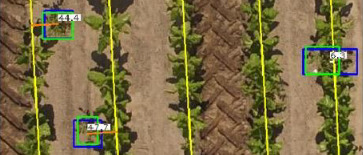
\includegraphics[width=0.7\linewidth]{img/biblio/feature-crop-row}
        \caption{Détection des rangs de culture et distance des adventices}
        \label{fig:03-feature-crop-row}
    \end{figure}
    
    
    \subsection{Propriétés de texture}  Finalement, les propriétés de texture sont plus vastes et incluent entre autres, des transformations de l'image (Fourier, Ondelettes, espaces colorimétriques, \dots), des propriétés spectrales ou encore des histogrammes. L'article \cite{mekhalfa2021supervised}, teste les propriétés de texture et de couleur sur des images RGB de soja. Les caractéristiques de couleur proposées, sont les moyennes et les écart-types des trois bandes de l'image des espaces colorimétriques RGB et HSV. En termes de propriétés de texture, c'est-à-dire une analyse des distributions spatiales des couleurs, l'article se repose sur les caractéristiques GLCM (Gray-Level Cooccurrence Matrix), d'Haralick et de LBP (Local Binary Pattern). D'après l'étude, les résultats reposant sur ces propriétés ont donné des taux de classification entre \SI{89.43}{\percent} et \SI{96.17}{\percent}. La figure \ref{fig:03-feature-color} ci-après montre différentes transformations qui peuvent être appliquées. À partir de ces nouvelles données des propriétés statistiques sont extraites, comme l'histogramme, les moyennes, etc.
    
    \begin{figure}[H]
        \centering
        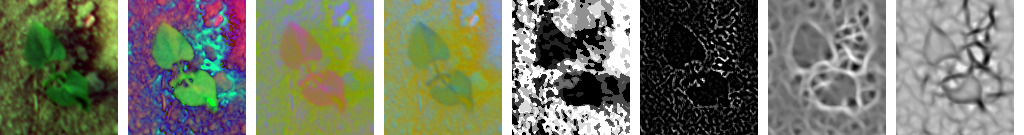
\includegraphics[width=\linewidth]{img/biblio/feature-colorspace}
        {\scriptsize De gauche à droite, les espaces colorimétriques RGB, HSV, YUB, et LAB, \\ puis les transformations LBP, Laplacian et les valeurs propre minimum et maximum de la matrice hessienne}
        \caption{Exemple de transformation d'une image de haricot}
        \label{fig:03-feature-color}
    \end{figure}
    
    
    %\begin{figure}
    %	\centering
    %	{\scriptsize (source: \cite{DBLP:journals/corr/abs-2103-14872})} \\
    %	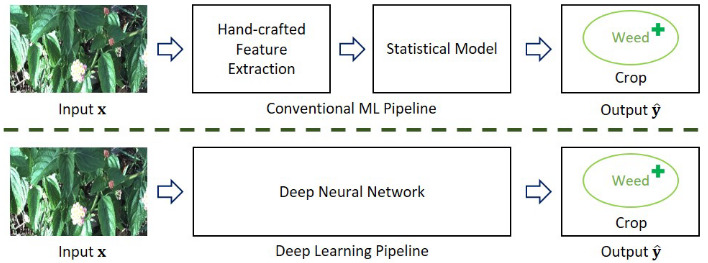
\includegraphics[width=0.7\linewidth]{img/biblio/synthezed-feature-classification-to-cnn}
    %	\caption{}
    %	\label{fig:03-synthezed-feature-classification-to-cnn}
    %\end{figure}
    
    \newpage
    \subsection{Robustesse des propriétés}
    
    % https://www.mdpi.com/2072-4292/13/3/531/htm
    % Review of Weed Detection Methods Based on Computer Vision
    % https://www.mdpi.com/2624-6511/3/3/39/htm
    % 
    
    Les articles de revue de \cite{wu2021review} et de \cite{smartcities3030039} recensent les propriétés qui ont été utilisées pour la discrimination des adventices. Ces articles montrent également, que pour obtenir des propriétés discriminantes, ces dernières doivent si possible être invariantes ; c'est-à-dire qu'elles ne changent pas de valeur face à des transformations de l'entrée, par exemple, la translation, la rotation, le changement d'échelle ou la couleur. Chaque type de propriété présente donc des avantages et des inconvénients \cite{wu2021review}. Le tableau suivant \ref{tab:03-feature-invariance} illustre les avantages et sources d'erreur de ces propriétés.
    
    \begin{table}[H]
        \centering
        {\scriptsize T=Translation ; R=Rotation ; S=Scale ; C=Color } \\
        %\rowcolors{0}{gray!10}{white}
        \begin{tabularx}{\linewidth}{l l X}
            \hline
            Propriété & Invariance & Source d'erreur \\
            \hline
            Texture & T+S 		& Illumination ; Ombres ; Bruit ; Mélange spectral \\
            Shape 	& T+R+C 	  	& Segmentation ; Occlusion ; Résolution \\
            Spatial & R+S+T+C	& Intra-rang ; Taux d'infestation \\
            \hline
        \end{tabularx}
        \caption{Invariance et sources d'erreurs pour ces trois types de propriétés}
        \label{tab:03-feature-invariance}
    \end{table}
    
    La similitude entre les adventices et les cultures rend difficile leur discrimination à partir de telles propriétés. C'est pourquoi, les chercheurs mélangent différentes sources d'information pour tirer les avantages de chacune d'elles, afin d'améliorer la précision et la robustesse du résultat. D'avantage de propriétés sont exposées dans le chapitre \ref{chap:feature-extraction} qui est dédié à l'extraction, l'étalonnage et la sélection de propriétés.
    
    \subsection{Apprentissage profond}
    % https://www.researchgate.net/publication/350143395_A_survey_of_deep_learning_techniques_for_weed_detection_from_images
    
    Dans l'approche par apprentissage profond, les réseaux de neurones convolutifs (CNN) sont populaires pour la reconnaissance et le traitement des images \cite{Hasan2021}. Un ensemble de filtres de convolution est utilisé pour transformer l'image et en extraire des caractéristiques discriminantes (textures, bords, formes). Pendant l'apprentissage, le CNN optimise les valeurs des filtres de convolution. Cette solution qui intègre la classification, permet de s'affranchir de l'extraction ``manuelle'' des propriétés telles que précédemment évoquée (texture, spatial, forme). Cette approche est de plus en plus utilisée \cite{Hasan2021} pour la discrimination des adventices. L'article de \cite{rs12244185} montre des taux de classification entre \SI{97.5}{\percent} et \SI{97.8}{\percent} pour l'identification des adventices dans une culture de maïs. Des architectures plus avancées \cite{reedha2021vision} montrent des taux de classification entre \SI{99.6}{\percent} et \SI{99.8}{\percent}.
    
    \begin{figure}[H]
        \centering
        %\rsource{\href{https://medium.com/mlearning-ai/convolutional-neural-networks-8ac43671642d}{medium.com}}
        \source{\cite{gao2016hep}}
        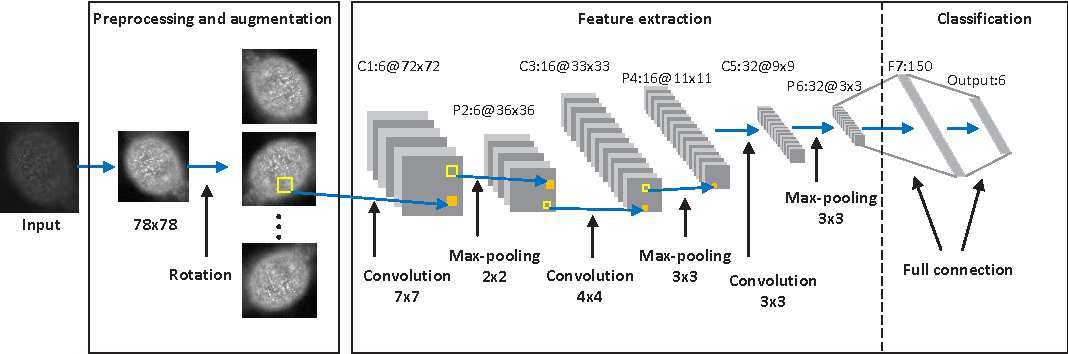
\includegraphics[width=.9\linewidth]{img/biblio/feature-cnn}
        \caption{Exemple d'un CNN pour la classification de cellule}
        \label{fig:03-feature-cnn}
    \end{figure}
    
    \newpage
    \section{Classification}
    
    La classification vise à identifier la catégorie à laquelle appartient un objet en se basant sur un ensemble de propriétés qui le décrit. Plus les données d'entrée sont variées (les descriptions de l'objet), plus il est ``facile'' pour la machine de trouver des modèles et plus le résultat est précis. De nombreux algorithmes d'apprentissage (machine learning), existent et se différencient en plusieurs domaines, dont \cite{Yuan2019} en proposent une taxonomie (figure \ref{fig:03-machine-learning-map}). Le but de cette section est simplement de montrer des exemples d'approches et non une présentation exhaustive des algorithmes. La plupart de ces méthodes de classification sont accessibles sous différents outils ou bibliothèques de programmation (shogun, mlpack, sklearn \cite{scikit-learn}, matlab \dots).
    
    \vfill
    \begin{figure}[H]
        \centering
        %\source{\href{https://vitalflux.com/great-mind-maps-for-learning-machine-learning/}{vitalflux.com},
        %    \href{https://vas3k.ru/blog/machine\_learning/}{vas3k.ru},
        %    \href{https://illya13.github.io/RL/reinforcement-learning.html}{illya13.github.io}}
        %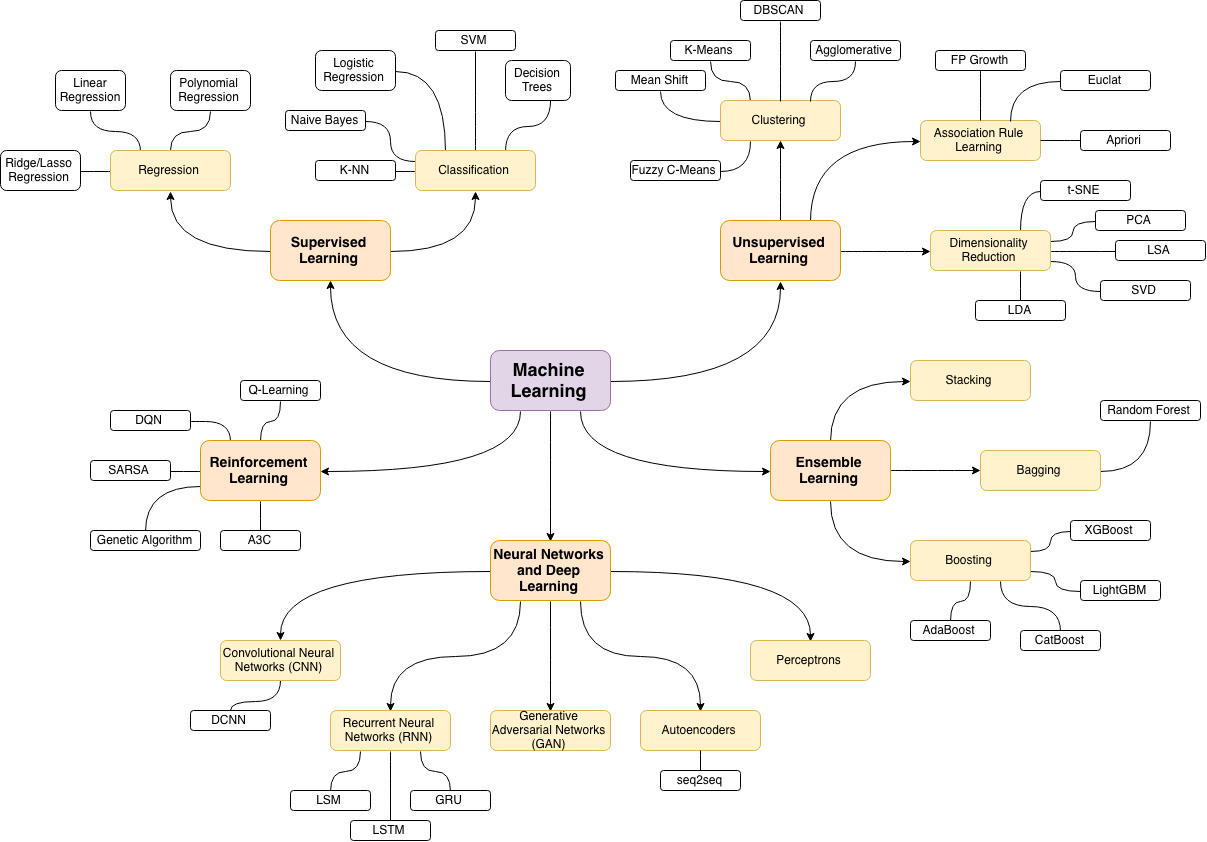
\includegraphics[width=0.9\linewidth]{img/biblio/machine-learning-map}
        %\source{Traduit de \cite{Yuan2019}}
        \footnotesize
        %\tikzset{
	ppblock/.style={
		rectangle,
		minimum size=6mm,
		very thick,
		draw=black!50,
		text centered,
		font=\ttfamily,
		minimum width=8em,
		minimum height=6mm,
		top color=white,
	},
	%
	figure/.style={
		rectangle,
		rectangle split,
		rectangle split parts=2,
		very thick,
		draw=black!50,
		text centered,
		append after command={
			\pgfextra
			\fill[top color=#1, bottom color=#1]
			(\tikzlastnode.one west) 
			[rounded corners] |- (\tikzlastnode.north) -| (\tikzlastnode.one east) 
			[sharp corners]   |- (\tikzlastnode.one split) -| cycle;
			\fill[top color=white, bottom color=#1]
			(\tikzlastnode.two west) 
			[rounded corners] |- (\tikzlastnode.south) -| (\tikzlastnode.two east)  
			[sharp corners]   |- (\tikzlastnode.one split) -| cycle;
			\endpgfextra
		},
	},
    splitted/.style={
        rectangle,
        rectangle split,
        rectangle split horizontal,
        rectangle split parts=2,
        very thick,
        draw=black!50,
        text centered,
        append after command={
            \pgfextra
            \fill[top color=white, bottom color=#1]
            (\tikzlastnode.south)
            [rounded corners] -| (\tikzlastnode.west) |- (\tikzlastnode.one north)
            [sharp corners]   -| (\tikzlastnode.one split) |- cycle;
            \fill[top color=white, bottom color=#1]
            (\tikzlastnode.two south)
            [rounded corners] -| (\tikzlastnode.east) |- (\tikzlastnode.north)
            [sharp corners]   -| (\tikzlastnode.one split) |- cycle;
            \endpgfextra
        },
    },
	%
	static/.style={ppblock, bottom color={black!20}},
	nonterminal/.style={ppblock, bottom color={blue!30}},
	terminal/.style={ppblock, bottom color={green!20}},
	algorithm/.style={ppblock, bottom color={yellow!50}},
	error/.style={ppblock, bottom color={red!20}},
	type/.style={ppblock, bottom color={red!20}},
	loss/.style={ppblock, dashed, bottom color={black!20}, font=\itshape},
	%
	tiny/.style={
		rounded rectangle,
		very thick,
		draw=black!50,
		top color=white,
		bottom color=red!20,
        text centered,
		font=\ttfamily,
	},
    operator/.style = {
        circle,
        scale=0.6,
        draw=black!50,
        top color=white,
        bottom color=red!20,
        font=\boldmath,
    },
	%
	skip loop/.style={to path={-- ++(0,#1) -| (\tikztotarget)}}
}

\begin{tikzpicture}[
    >=stealth',thick,
    tip/.style={->,shorten >=0.007pt},
    filled/.style = {fill=circle area, draw=circle edge, thick},
    outline/.style = {draw=circle edge, thick},
    F/.style = {
        draw, fill=white, inner sep=7mm, fit=(current bounding box), drop shadow, node contents={}
    },
    E/.style = {
        rectangle,
        minimum size=1cm,
        text width=2.5cm,
        outline
    },
    G/.style = {rectangle},
    every text node part/.style={align=center},
    scale=0.8
]
    \definecolor{tempcolor}{rgb}{1,1,1}
    \colorlet{circle edge}{black!50}
    \colorlet{circle area}{black!20}

    \coordinate (a) at (-2cm,-1.5cm);
    \coordinate (c) at ( 0cm, 2cm);
    \coordinate (d) at ( 2cm,-1.5cm);
    \coordinate (e) at (0cm,-0.25cm);
    
    \node[E, fill=green!20, xshift=-2.8cm]  at (a) {\scriptsize SVM, KNN, RF \\ AdaBoost \\[-0.5em] \dots};
    \node[E, fill=red!20, xshift= 2.8cm]   at (c) {\scriptsize PCA, K-means \\ DBSCAN \\[-0.5em] \dots};
    \node[E, fill=blue!20, xshift= 2.8cm] at (d) {\scriptsize Q-Learning \\ AC, A3C \\[-0.5em] \dots};

    \draw[filled, fill=green!20, outline] (a) circle (2.cm);
    \draw[filled, fill=red!20, outline] (c) circle (2.cm);
    \draw[filled, fill=blue!20, outline] (d) circle (2.cm);
    \draw[outline, fill opacity=0.5, fill=white] (e) circle (1.8cm);
    \draw[outline, pattern=north west lines, pattern color=black!30] (e) circle (1.8cm);
    
    \node[G, xshift=-0.2cm, yshift=-0.2cm, rotate=-45] at (a) {Apprentissage \\ supervisé};
    \node[G, xshift= 0.2cm, yshift=-0.2cm, rotate= 45] at (d) {Apprentissage \\ par renforcement};
    \node[G, xshift= 0.0cm, yshift= 0.4cm] at (c) {Apprentissage \\ non-supervisé};
    \node[G] at (e) { \textbf{Apprentissage} \\ \textbf{Profond}};
    
    \scoped[on background layer] \node (a) [F];
    
    \node[below left] at (a.north east) {Apprentissage Machine};
    
\end{tikzpicture}
        %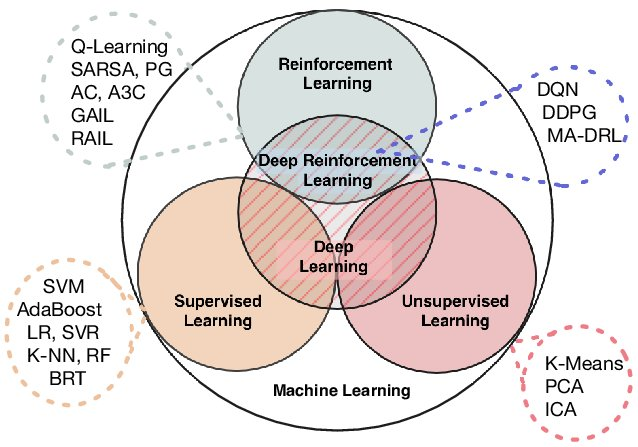
\includegraphics[width=0.7\linewidth]{img/biblio/machine-learning-map-2}
        \caption{Taxonomie des algorithmes d'apprentissage machine}
        \label{fig:03-machine-learning-map}
    \end{figure}
    \vfill
    
    \subsection{Classification supervisée}
    
    L'objectif de la classification supervisée est de définir des règles qui permettent de classer les objets à partir de variables qualitatives ou quantitatives. Les règles de classification sont apprises en utilisant un échantillon d'apprentissage, contenant les variables discriminantes et leurs classements connus. La classification supervisée est une approche standard et privilégiée par la majorité des études, tout comme en agriculture de précision \cite[p.~37]{MRNL2016} (knn, tree, svm, \dots). Les réseaux de neurones \cite{DBLP:journals/corr/abs-1806-03412,DBLP:journals/corr/abs-1002-4046, Koot891024465110} (ann, cnn, \dots) font partie des méthodes de classification supervisée. La difficulté de cette méthode réside principalement dans la conception du jeu de données d'apprentissage.
    
    % Cette étape est effectuée manuellement, elle est donc coûteuse, souvent imprécise et incomplète. De plus, en agriculture de précision, il est difficile d'obtenir des propriétés stables, ce qui rend difficile l'utilisation d'algorithmes basés sur un apprentissage supervisé. Les différences de condition d'acquisition peuvent modifier les étapes de segmentation et les propriétés extraites. Si bien que, une classification apprise sur un jeu de données est difficilement transposable à d'autres jeux de données. Quelques méthodes de classification sont présentées ci-dessous.
    
    \newpage
    \subsubsection{Approche Bayésienne} Ici le but est de trouver en amont la distribution des classes afin de prédire l'appartenance de nouvelles données à partir d'une fonction de densité de probabilité connue. L'objectif est de réduire la probabilité d'erreur de classement \cite{dunsmore1966bayesian}. Lorsqu'une donnée est recouverte par plusieurs classes, c'est la classe dont la probabilité est la plus forte qui prend l'avantage. En cas d'égalité de probabilité, il n'y a pas de méthodes pour lever l'incertitude ce qui provoque une erreur de classification, comme dans le diagramme ci-dessus (figure \ref{fig:03-classification-bayes}). %, l'approche Bayésienne est insuffisamment.
    
    \begin{figure}[H]
        \centering
        %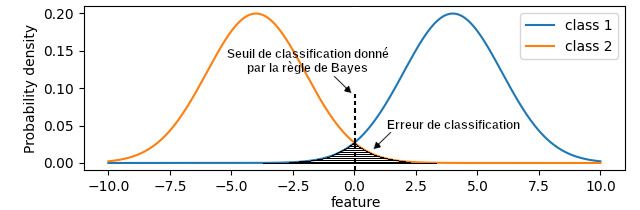
\includegraphics[height=4.cm]{img/biblio/classification-bayes}
        
\usepgfplotslibrary{fillbetween}
\pgfplotsset{compat=1.12}

\pgfmathdeclarefunction{gauss}{3}{%
    \pgfmathparse{1/(#3*sqrt(2*pi))*exp(-((#1-#2)^2)/(2*#3^2))}%
}

% GAUSSIANs: confidence level
\begin{tikzpicture}[>=stealth',thick,tip/.style={->,shorten >=0.007pt},]

\def\q{5.5};
\def\B{4};
\def\S{7};
\def\Bs{1.00};
\def\Ss{1.00};
\def\xmax{\S+3.2*\Ss};
\def\ymin{{-0.15*gauss(\B,\B,\Bs)}};

\begin{axis}[height=6cm,width=\linewidth,every axis plot post/.append style={
    mark=none,domain={-0.05*(\xmax)}:{1.08*\xmax},samples=80,smooth},
xmin={-0.1*(\xmax)}, xmax=\xmax,
ymin=\ymin, ymax={1.1*gauss(\B,\B,\Bs)},
axis line style=thick,
enlargelimits=upper, % extend the axes a bit to the right and top
ticks=none,
%xlabel={propriété},
ylabel={densité de probabilité},
%every axis x label/.style={at={(current axis.right of origin)},anchor=north west},
]

% plots
\addplot[name path=B,very thick,black!10!teal] {gauss(x,\B,\Bs)};
\addplot[name path=S,very thick,black!10!orange ] {gauss(x,\S,\Ss)};
\addplot[black,dashed,name path=Q,thick]
coordinates {(\q, {0.90*gauss(\B,\B,\Bs)}) (\q, \ymin)}
node[below=2pt,anchor=south west] {\scriptsize \textbf{Seuil de classification donné par Bayes}};

% fill
\path[name path=xaxis] (0,0) -- (\xmax,0); % \pgfkeysvalueof{/pgfplots/xmin}
\addplot[white!50!teal] fill between[of=xaxis and B, soft clip={domain=\q:\xmax}];
\addplot[white!50!orange]  fill between[of=xaxis and S, soft clip={domain=0:\q}];

% labels
\node[above,      black!20!teal] at (1.0*\B,{gauss(\B,\B,\Bs)}) {\scriptsize \textbf{Données de Classe 1}};
\node[above right,black!20!orange ] at (0.82*\S,{gauss(\S,\S,\Ss)}) {\scriptsize \textbf{Données de Classe 2}};
%\node[above left, black!20!red ] at ({0.8*\q},{gauss(1.07*\q,\B,\Bs)}) {\strut$\beta$};
%\node[above right,black!20!blue] at ({1.1*\q},{gauss(1.07*\q,\B,\Bs)}) {\strut$\alpha$};

\node[above left] (I) at ({\B*1.38},{0.27*gauss(\B,\B,\Bs)}) {\scriptsize \textbf{Erreur de classification}};

\draw[->] (I.south) to ({\B/2+\q/1.7}, 0.035);
\draw[->] (I.south) to ({\S/2+\q/2.3}, 0.035);

\end{axis}
\end{tikzpicture}
        \caption{Règle de décision de Bayes}
        \label{fig:03-classification-bayes}
    \end{figure}
    
    La règle de décision de Bayes constitue en réalité la limite optimale de tout système de classification. Cette limite est théorique : face à un problème réel, les distributions des classes sont inconnues, ainsi que les probabilités a posteriori. Les différentes méthodes de résolution peuvent seulement en fournir des estimations. Cette erreur théorique constitue une borne infranchissable qui représente d'une certaine manière la difficulté intrinsèque du problème.
    
    \subsubsection{K Plus Proche Voisins} L'algorithme des KPPV ou KNN (\textit{K Nearest Neighbor}) est un algorithme de classification et de régression. Dans cette méthode, on calcule la distance entre le point à classer et l'ensemble des autres points de toutes les classes d'une base de données de référence, on prend les $k$ plus proches et la classe majoritaire identifie l'objet. C'est une méthode de référence lorsque les connaissances préalables sur la distribution des données sont insuffisantes \cite{peterson2009k}. La figure \ref{fig:03-classification-knn} montre la classification du point noir en fonction de $K$. Quand $K$ est pair il n'y a pas de classe majoritaire, ce qui implique une frontière d'indécision (visible en blanc, image central) et une heuristique supplémentaire peut être utilisée, par exemple en utilisant un voisin de moins (image de droite). Le choix de $K$ et de l'heuristique est difficile. Si K est trop petit, la classification est trop sensible au bruit (image de gauche K=1). À l'inverse, si K est trop grand, la classification peut-être erronée par une trop grande zone de décision.
    
    \vspace{-0.5em}
    \begin{figure}[H]
        \centering
        \begin{subfigure}[b]{0.3\textwidth}
            \centering
            \caption*{$K=1$}
            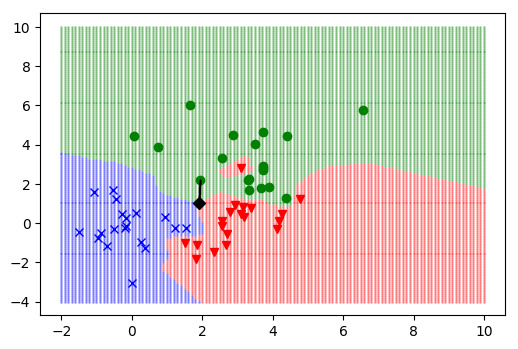
\includegraphics[width=\linewidth]{img/biblio/classification-knn-1}
        \end{subfigure}
        \begin{subfigure}[b]{0.3\textwidth}
            \centering
            \caption*{$K=4$}
            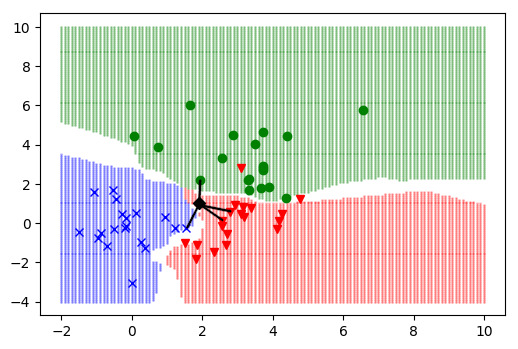
\includegraphics[width=\linewidth]{img/biblio/classification-knn-4}
        \end{subfigure}
        \begin{subfigure}[b]{0.3\textwidth}
            \centering
            \caption*{$K=4+heuristique$}
            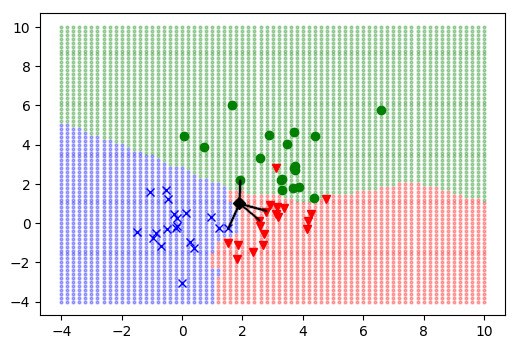
\includegraphics[width=\linewidth]{img/biblio/classification-knn-4-decrement}
        \end{subfigure}
        \caption{Classification KNN : influence de K et de l'heuristique}
        \label{fig:03-classification-knn}
    \end{figure}
    
    \newpage
    \subsubsection{Perceptron} Le perceptron est le modèle de base des réseau de neurones \cite{rosenblatt1958perceptron}. Cet algorithme aide à trouver une droite de séparation entre deux sets de données par descente de gradient afin d'établir une classification des données entrées. Le perceptron recherche l'hyperplan séparateur entre deux classes de points ($-1$ et $+1$). L'hyperplan est défini par $f(x) = \sum_{i=1}^n w_i x_i + b = \langle w, x \rangle + b$ avec $w$ le vecteur orthogonal à l'hyperplan, $b$ le déplacement à l'origine et $n$ le nombre de dimensions. Lorsque davantage de classes sont évaluées, il est possible d'obtenir la classification grâce à plusieurs droites de séparation, une par paire de classe. Visible sur la figure \ref{fig:03-classification-perceptron}, dont les axes correspondent à des propriétés quelconques.
    
    \begin{figure}[H]
        \centering
        
        \begin{subfigure}[b]{0.3\textwidth}
            \centering
            \caption*{2 classes}
            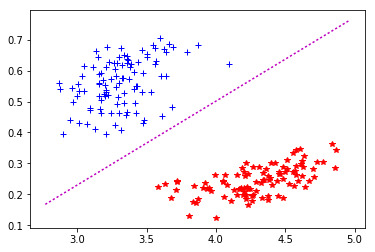
\includegraphics[width=\linewidth]{img/biblio/classification-perceptron-2}
        \end{subfigure}
        \hspace{0.1\linewidth}
        \begin{subfigure}[b]{0.3\textwidth}
            \centering
            \caption*{3 classes}
            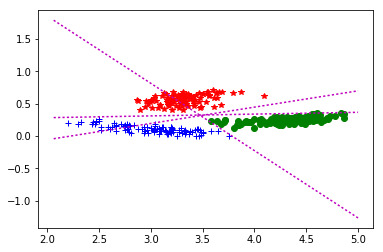
\includegraphics[width=\linewidth]{img/biblio/classification-perceptron-3}
        \end{subfigure}
        \caption{Perceptron}
        \label{fig:03-classification-perceptron}
    \end{figure}
    
    
    \subsubsection{Arbre de décision} L'objectif est de créer un modèle qui prédit la valeur d'une variable cible en apprenant des règles de décision simples déduites des caractéristiques des données. En combinant ces règles de décision, une structure arborescente est construite. Les feuilles finales représentent les classes et les branches représentent les conditions sur les caractéristiques qui mènent aux classes. Dans la figure suivante \ref{fig:03-classification-decision-tree}, en s'appuyant sur de la bibliographie, un arbre de décision peut-être manuellement construit pour classer des pixels en 3 classes (eau, sol, végétation) à partir d'un indice de végétation tel que le NDVI (voir section \ref{sec:vegetation-indices}). Si celui-ci est inférieur à 0 alors c'est de l'eau, sinon, c'est ``autre chose'' et on continue. Cette approche peut être automatisée, pour chaque variable à disposition, une métrique est utilisée pour définir celle qui divise au mieux les ensembles (Gini Impirity / Information Gain / Variance / \dots). Ensuite, la valeur de seuillage peut-être apprise par régression pour obtenir la meilleure séparation de deux ensembles. Cette solution présente l'avantage de donner l'importance aux propriétés et aux décisions associées, ce qui permet d'expliquer facilement la démarche de classification.
    
    \begin{figure}[H]
        \centering
        %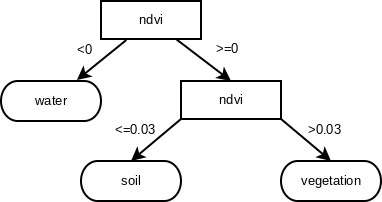
\includegraphics[height=4cm]{img/biblio/classification-decision-tree}
        \tikzset{
	base/.style = {
		rectangle, rounded corners,
		draw=black,
		top color=white,
		bottom color=black!20,
		minimum width=3.5cm,
		minimum height=1.0cm,
		text centered,
		font=\ttfamily
	},
	every node/.style={
		font=\ttfamily,
		scale=0.8
	},
	% Specifications for style of nodes:
	activityStarts/.style = {
		base,
		fill=blue!30,
		bottom color=blue!20,
	},
	startstop/.style = {
		base,
		fill=red!30
	},
	activityRuns/.style = {
		base,
		fill=green!30
	},
	process/.style = {
		base,
		%minimum width=2.5cm,
		fill=orange!15,
		bottom color=green!20,
		font=\ttfamily
	},
	%
	point/.style={coordinate},
	draw=black!75,
	tip/.style={->,shorten >=0.007pt},
	every join/.style={rounded corners},
	align=center,
}

\begin{tikzpicture}[
		>={Latex[width=2mm,length=2mm]},
		>=latex,thick,
		node distance=1.5cm,
    ]
    
    \node (p1)    [process, xshift= 0em, yshift=-0em, minimum height=0.8cm]           {NDVI};
    \node (p2)    [startstop, xshift=-5em, yshift=-5em, minimum height=0.8cm]         {water};
    \node (p3)    [process, xshift= 5em, yshift=-5em, minimum height=0.8cm]           {NDVI};
    \node (p4)    [startstop, xshift= 0em, yshift=-10em, minimum height=0.8cm]        {soil};
    \node (p5)    [startstop, xshift= 10em, yshift=-10em, minimum height=0.8cm]       {vegetation};

    
	\begin{scope}[->,rounded corners=2mm]
        \draw[->] (p1) -- node [text width=1cm,midway, left=0.0cm] {$<0$} (p2);
        \draw[->] (p1) -- node [text width=1cm,midway, right=0.2cm] {$\geq0$} (p3);
        \draw[->] (p3) -- node [text width=1.5cm,midway, left=0.0cm] {$<0.03$} (p4);
        \draw[->] (p3) -- node [text width=1.5cm,midway, right=0.2cm] {$\geq0.03$} (p5);
	\end{scope}
    
\end{tikzpicture}
        \caption{Arbre de décision simple en agriculture de précision}
        \label{fig:03-classification-decision-tree}
    \end{figure}
    
    \newpage
    \subsection{Classification non-supervisée}
    
    Les méthodes de classification non-supervisées, sont souvent basées sur des mesures de distance pour agglomérer les individus proches, sans avoir besoin de connaître la classe de l'individu a priori. Cette approche propose deux grands intérêts, en agriculture de précision (i) l'absence de base d'apprentissage annotée et (ii) de s'abstraire des conditions d'acquisition, qui sont alors plus ``uniformes'', par exemple au sein de l'image. Dû à la faible séparabilité des propriétés extraites entre culture et adventice, cette solution n'est pas encore utilisable pour cette tâche. Cependant, elle reste applicable à la séparation sol/végétation, dont le seuillage \textit{Otsu} présenté précédemment en est un exemple de classification binaire.
    
    %Quelques articles proposent une classification non-supervisé à partir d'informations à posteriori, notamment par la détection des rangs \cite{rs10050761} (SVM + spectral + spatial + composante connexe) \cite{DBLP:journals/corr/abs-1805-12395} (CNN + superpixel + multiscale). Cela permet de créer deux ensembles (culture et adventice) sur la base de la probabilité d'appartenance. Les cultures sont majoritairement dans le rang, et les adventices dans l'inter-rang. Les défauts de cette méthode résident sur deux points, la présence de bruit, i.e la présence d'adventice dans le rang et inversement. Mais aussi sur la limite du type de culture (sarclé), ainsi que le stade de développement i.e lorsque la couverture des cultures recouvre l'inter-rang la méthode n'est plus adaptée.
    
    \paragraph{K-means} L'algorithme des k-means permet de regrouper les individus au sein de groupes (clusters) distincts en utilisant une mesure de distance. Pour ce faire, on fixe des centres de groupes de départ aléatoirement en quantité déterminée. Ce sont des informations à priori que nous avons sur les données. Pour chaque donnée, on associe le centre le plus proche puis on recalcule les nouveaux centres des clusters ainsi formés. Cette étape est ré-itérée tant qu'il n'y a pas convergence, c'est-à-dire tant que les centres de chaque groupe ne sont pas stabilisés (avec une tolérance). À l'issue de son exécution, l'algorithme des kmeans a alors associé chaque donnée à un groupe.
    
    \vspace{-0.5em}
    \begin{figure}[H]
        \centering
        \begin{subfigure}[b]{0.3\textwidth}
            \centering
            \caption*{$K=2$}
            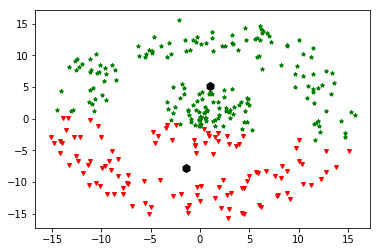
\includegraphics[width=\linewidth]{img/biblio/classification-kmean-2}
        \end{subfigure}
        \begin{subfigure}[b]{0.3\textwidth}
            \centering
            \caption*{$K=3$}
            \includegraphics[width=\linewidth]{img/biblio/classification-kmean-3}
        \end{subfigure}
        \begin{subfigure}[b]{0.3\textwidth}
            \centering
            \caption*{$K=5$}
            \includegraphics[width=\linewidth]{img/biblio/classification-kmean-4}
        \end{subfigure}
        \caption{Algorithme de classification K-Mean}
        \label{fig:03-classification-kmean-2}
    \end{figure}
    \vspace{-0.5em}
    
    \paragraph{DBSCAN} L'algorithme considère les clusters comme des zones de haute densité séparées par des zones de faible densité. Deux paramètres, $N$ et $\epsilon$, définissent formellement ce que signifie ``dense''. On prend le premier individu et on vérifie combien de voisins sont autour de lui à une distance maximale de $\epsilon$, si le nombre de voisins est inférieur à $N$ c'est un ``bruit'', sinon il fait partie d'un cluster. On crée alors une catégorie en y associant les points par propagation. On répète l'opération pour chaque individu non traité. Donc prendre un $N$ plus élevé ou un $\epsilon$ plus faible, indiquent une plus grande densité nécessaire pour former un cluster. La méthode, illustrée sur la figure \ref{fig:03-classification-dbscan} montre en orange le bruit, en vert les premiers individus testés et en bleu ceux associés par propagation.
    
    \begin{figure}[H]
        \centering
        \source{\cite{Khater2020}}
        \includegraphics[width=0.7\linewidth]{img/biblio/classification-dbscan}
        \caption{Illustration de la méthode de clustering DBSCAN}
        \label{fig:03-classification-dbscan}
    \end{figure}
    
    \newpage	
    \subsection{Classification semi-supervisée}
    
    Un exemple est l'apprentissage d'un classificateur sur une petite base de données annotée. Ce dernier pourrait alors être optimisé dans le temps, à chaque nouvelle observation. Une littérature exhaustive sur les modèles d'apprentissage semi-supervisés a été effectuée par \cite{Zhu06semi-supervisedlearning}. Un autre exemple d'apprentissage semi-supervisé est le co-apprentissage, dans lequel deux classificateurs apprennent un ensemble de données, mais en utilisant chacun un ensemble de caractéristiques différentes, idéalement indépendantes.
    
    \paragraph{Connaissance a priori} L'étude \cite{8206403} met en place une méthode de détection d'adventices semi-supervisée ($80-\SI{95}{\percent}$) dans laquelle ils exploitent le fait que la plupart des cultures sont plantées en rangées avec un espacement similaire le long du rang, ce qui peut être utilisé pour améliorer un classificateur existant. Cette même connaissance a été utilisée par \cite{rs10050761}. Une segmentation \textit{Otsu} est utilisée pour séparer le sol de la végétation. Une détection de rang permet ensuite de créer un sous-ensemble d'apprentissage pour la discrimination culture/adventice, en utilisant des informations spectrales. Finalement, la classe de chaque composante connexe est déduite à partir de ces deux classifications (rang+spectre). Les résultats ($75-\SI{85}{\percent}$) sont fortement dépendants de la résolution des images qui implique un fort mélange spectral et homogénéise les composantes connexes. Cette approche semble difficilement applicable en présence d'une densité importante de plantes. 
    
    \paragraph{Espace latent} À partir d'un ensemble minimal de connaissances, la construction d'un espace latent qui représente ces individus peut être construit. On cherche alors à diminuer la variance intra-classe tout en maximisant la distance inter-classe, utilisée comme fonction de perte. À chaque nouvelle observation, l'individu est projeté dans l'espace latent et associé au cluster le plus proche. Quand suffisamment de nouvelles connaissances sont apportées, on peut renforcer la représentation de cette espace latent en minimisant une nouvelle fois la fonction de perte. Pour construire l'espace latent, différentes méthodes peuvent être utilisées, telles que l'apprentissage profond \cite{Kamnitsas2018}. En agriculture de précision, on peut apprendre l'espace latent à partir d'un petit échantillon et à chaque nouvelle image, les cultures et les adventices précédemment classées sont utilisées pour optimiser l'espace latent, ce qui permet de prendre en considération les changements d'illumination ou de stade de développement des cultures.
    
    \begin{figure}[H]
        \centering
        \source{\cite{Kamnitsas2018}}
        \includegraphics[width=0.7\linewidth]{img/biblio/classification-latent-space}
        \caption{Optimisation de l'espace latent}
        \label{fig:03-classification-latent-space}
    \end{figure}
    
    %\newpage
    %
    %\subsection{Selection des meilleurs propriétées}
    %\par La sélection des propriétés se fait en général soit manuellement après visualisation notamment grâce à un \og scatter plot \fg, pour visualiser le niveau d'inter-corrélation des variables, soit par l'utilisation d'algorithmes de réduction de dimensions (PCA, SVD, RandomForest,\dots) \ref*{fig:03-machine-learning-map}. Différents critères sont alors utilisés pour définir les meilleurs propriétés tels-que :
    %\\
    %\begin{itemize}
    %	\item Choisir les propriétés en fonction de leur "séparabilité" des classes \cite{Fukunaga:1990:ISP:92131}.
    %	\item Rejeter les propriétés trop asymétriques, trop corrélées \cite{Lerski1993MRIT}
    %	\item Selectioner les propriétés les plus discriminantes \cite{Lerski1993MRIT}
    %\end{itemize}
    %
    %\par Les url suivantes expliquent en détail la sélection automatique de propriétés : \\
    %
    %\begin{itemize}
    %	\item \url{https://blog.datadive.net/selecting-good-features-part-i-univariate-selection/}
    %	\item \url{https://blog.datadive.net/selecting-good-features-part-ii-linear-models-and-regularization/}
    %	\item \url{https://blog.datadive.net/selecting-good-features-part-iii-random-forests/}
    %	\item \url{https://blog.datadive.net/selecting-good-features-part-iv-stability-selection-rfe-and-everything-side-by-side/}
    %\end{itemize}
    
    %\newpage
    %\subsection{Performances dans la littérature}
    %
    %Les tableaux ci après présentent les performances de classification de différentes méthodes décrites dans la littérature en proxy-detection. Néanmoins dans la bibliographie examinée, il n'est pas toujours stipulé toutes les étapes, les propriétés analysées ou les cultures visées. Principalement lorsque l'article fait lui-même des références à d'autres études antérieures.
    %
    %\noindent
    %\begin{multicols}{2}
    %	\noindent \vspace{1em}
    %	\begin{minipage}[t]{\linewidth}
    %		\par \cite[p.52-54]{MRNL2016} biblio donnée \\
    %		\begin{tabularx}{\linewidth}{|X|c|c|}
    %			\hline
    %			\textbf{Méthode} & \textbf{culture} & \textbf{perf} \\
    %			\hline\hline
    %			Forme & maïs & 84\% \\
    %			HSI & -- & 93-98\% \\
    %			Spectral & colza fleur & 87.2\% \\
    %			Spectral & maïs & 99\% \\
    %			Spectral & betterave & 93\% \\
    %			Spectral & blé & 91\% \\
    %			Spectral & autres & 52-72\% \\
    %			Spectral+Spatial & maïs & 86-89\% \\
    %			Spectral+Spatial & tournesol & 96.33\% \\
    %			\hline
    %		\end{tabularx}
    %	\end{minipage}
    %	
    %	\noindent \vspace{1em}
    %	\begin{minipage}[t]{\linewidth}
    %		\par \cite[p.55-58]{MRNL2016} biblio classification \\
    %		\begin{tabularx}{\linewidth}{|X|c|c|}
    %			\hline
    %			\textbf{Méthode} & \textbf{culture} & \textbf{perf} \\
    %			\hline\hline
    %			Bayes & blé-crucifère & 85-92\% \\
    %			Vraisemblence & blé-crucifère & 85.8-91.3\% \\
    %			K-means & betterave & 57-76\% \\
    %			K-means & betterave & 77.2-94.1\% \\
    %			CART & betterave & 70-83\% \\
    %			CART & maïs & 60-68\% \\
    %			ANN & betterave & 80.1-91.4\% \\
    %			CNN radial & blé & 98.7\% \\
    %			Perceptron & -- & 96.7\% \\
    %			SVM radial & tournesol & 97.3\% \\
    %			\hline
    %		\end{tabularx}
    %	\end{minipage}
    %	\noindent \vspace{1em}
    %	\begin{minipage}[t]{\linewidth}
    %		\par \cite[p.234]{MRNL2016} Mise en place : NDVI \\
    %		\begin{tabularx}{\linewidth}{|X|c|c|}
    %			\hline
    %			\textbf{Méthode} & \textbf{culture} & \textbf{perf} \\
    %			\hline\hline
    %			LDA & *cotylédone & 81\% \\
    %			QDA & *cotylédone & 82\% \\
    %			Mahalanobis & *cotylédone & 81\% \\
    %			SVM poly & *cotylédone & 81\% \\
    %			SVM RBF & *cotylédone & 81\% \\
    %			SVM sigmoide & *cotylédone & 80\% \\
    %			\hline
    %		\end{tabularx}
    %	\end{minipage}
    %	\noindent \vspace{1em}
    %	\begin{minipage}[t]{\linewidth}
    %		\par \cite[p.235]{MRNL2016} Centre composante \\
    %		\begin{tabularx}{\linewidth}{|X|c|c|}
    %			\hline
    %			\textbf{Méthode} & \textbf{culture} & \textbf{perf} \\
    %			\hline\hline
    %			LDA & *cotylédone & 79\% \\
    %			QDA & *cotylédone & 76\% \\
    %			Mahalanobis & *cotylédone & 74\% \\
    %			SVM poly & *cotylédone & 78\% \\
    %			SVM RBF & *cotylédone & 79\% \\
    %			SVM sigmoide & *cotylédone & 78\% \\
    %			\hline
    %		\end{tabularx}
    %	\end{minipage}
    %	\noindent \vspace{1em}
    %	\begin{minipage}[t]{\linewidth}
    %		\par \cite{Koot891024465110} Proprités RGB + multispectral
    %		
    %		\begin{tabularx}{\linewidth}{|c|X|c|c|}
    %			\hline
    %			\textbf{Méthode} & \textbf{culture} & \textbf{acc} & \textbf{miss} \\
    %			\hline\hline
    %			LDA & radis & 98\% & 8\% \\
    %			ANN & radis & 100\% & 0\% \\
    %			LDA & beterave & 90\% & 22\% \\
    %			QDA & carrot & 57-80\% & 15-25\% \\
    %			LDA & patate & 87\% & -- \\
    %			QDA & patate & 82\% & -- \\
    %			ANN & patate & 99\% & -- \\
    %			\hline
    %		\end{tabularx}
    %	\end{minipage}
    %	\noindent \vspace{1em}
    %	\begin{minipage}[t]{\linewidth}
    %		\par \cite[p.~9335]{rs70709325} classification supervisée \\
    %		\begin{tabularx}{\linewidth}{|X|c|c|}
    %			\hline
    %			\textbf{Méthode} & \textbf{culture} & \textbf{perf} \\
    %			\hline\hline
    %			SVM & 9 classe & 88\% \\
    %			SVM & 6 classe & 94\% \\
    %			Overall Accuracy & 6 classe & 80.1\% \\
    %			Overall Accuracy & 10 classe & 90.7\% \\
    %			\hline
    %		\end{tabularx}
    %	\end{minipage}
    %	\noindent \vspace{1em}
    %	\begin{minipage}[t]{\linewidth}
    %		\par Rice classification\cite{Rice2010} \\
    %		\begin{tabularx}{\linewidth}{|X|c|c|}
    %			\hline
    %			\textbf{Méthode} & \textbf{culture} & \textbf{perf} \\
    %			\hline\hline
    %			CNN & -- & 98\% \\
    %			Likelihood & 7 classes & 78-79\% \\
    %			Likelihood & 11 classes & 84.7\% \\
    %			Minimum distance classifier & 2 classes & 95.7\% \\
    %			\hline
    %		\end{tabularx}
    %	\end{minipage}
    %\end{multicols}
    
    %Il convient de même, de prêter une attention certaine a ces résultats dont les métriques d'évaluations ne sont pas concordantes.
    %Par exemple certaines méthodes ce base sur une classification de pixel tandis que d'autres sur des composantes connexes.
    %Nous ne pouvons donc pas utiliser ces résultats bibliographiques pour comparer les algorithmes, mais permet simplement de ce donner une idée des possibilités.
    
    \newpage
    \section{Métriques d'évaluation}
    
    Pour évaluer une méthode (classification, régression, \dots), de nombreuses métriques sont utilisées dans la littérature \cite{hossin2015review,di2008review}. En fonction du problème étudié et de la nature de l'information traitée, les métriques utilisables pour estimer les performances d'un modèle sont différentes (Figure \ref{fig:03-model-performances}). Ainsi dans cette section chaque partie % présenteras un ensemble de métrique associée à un problème spécifique.
    s'intéressera à un problème spécifique et présentera un ensemble de métriques permettant de le traiter.
    
    %Au-delà des traditionnels indicateurs statistiques tels que le Mean Square Error (MSE) ou Root mean Square Error (RMSE), la plupart des métriques utilisées pour la classification proviennent de la matrice de confusion qui donne une vue globale des performances d'une méthode. %Les principaux indicateurs sont résumés dans le tableau suivant.
    
    \begin{figure}[H]
        \centering
        
  \tikzset{
	ppblock/.style={
		rectangle,
		minimum size=6mm,
		very thick,
		draw=black!50,
		text centered,
		font=\ttfamily,
		minimum width=8em,
		minimum height=6mm,
		top color=white,
	},
	%
	figure/.style={
		rectangle,
		rectangle split,
		rectangle split parts=2,
		very thick,
		draw=black!50,
		text centered,
		append after command={
			\pgfextra
			\fill[top color=#1, bottom color=#1]
			(\tikzlastnode.one west) 
			[rounded corners] |- (\tikzlastnode.north) -| (\tikzlastnode.one east) 
			[sharp corners]   |- (\tikzlastnode.one split) -| cycle;
			\fill[top color=white, bottom color=#1]
			(\tikzlastnode.two west) 
			[rounded corners] |- (\tikzlastnode.south) -| (\tikzlastnode.two east)  
			[sharp corners]   |- (\tikzlastnode.one split) -| cycle;
			\endpgfextra
		},
	},
    splitted/.style={
        rectangle,
        rectangle split,
        rectangle split horizontal,
        rectangle split parts=2,
        very thick,
        draw=black!50,
        text centered,
        append after command={
            \pgfextra
            \fill[top color=white, bottom color=#1]
            (\tikzlastnode.south)
            [rounded corners] -| (\tikzlastnode.west) |- (\tikzlastnode.one north)
            [sharp corners]   -| (\tikzlastnode.one split) |- cycle;
            \fill[top color=white, bottom color=#1]
            (\tikzlastnode.two south)
            [rounded corners] -| (\tikzlastnode.east) |- (\tikzlastnode.north)
            [sharp corners]   -| (\tikzlastnode.one split) |- cycle;
            \endpgfextra
        },
    },
	%
	static/.style={ppblock, bottom color={black!20}},
	nonterminal/.style={ppblock, bottom color={blue!30}},
	terminal/.style={ppblock, bottom color={green!20}},
	algorithm/.style={ppblock, bottom color={yellow!50}},
	error/.style={ppblock, bottom color={red!20}},
	type/.style={ppblock, bottom color={red!20}},
	loss/.style={ppblock, dashed, bottom color={black!20}, font=\itshape},
	%
	tiny/.style={
		rounded rectangle,
		very thick,
		draw=black!50,
		top color=white,
		bottom color=red!20,
        text centered,
		font=\ttfamily,
	},
    operator/.style = {
        circle,
        scale=0.6,
        draw=black!50,
        top color=white,
        bottom color=red!20,
        font=\boldmath,
    },
	%
	skip loop/.style={to path={-- ++(0,#1) -| (\tikztotarget)}}
}
  \vspace{-1em}
  \begin{tikzpicture}[
    >=stealth',thick,
    tip/.style={->,shorten >=0.007pt},
    every node/.style={scale=0.75, minimum width=10em},
  ]
  \matrix[column sep=8mm, row sep=4mm, align=center] {
   \node (X)     [terminal]   {Données};        &
   \node (M)     [algorithm]   {Modèle};        &
   \node (p)     [nonterminal]   {Prédictions};       &
   \node (E)     [loss]   {Performances}; &
   \node (y)     [terminal]   {Références};        \\
  };
  
  \draw[->] (X) to (M);
  %\draw[->] (y) to (M);
  \draw[->] (M) to (p);
  
  \draw[->] (y) to (E);
  \draw[->] (p) to (E);
\end{tikzpicture}
        \caption{Evaluation des performances d'un modèle après apprentissage}
        \label{fig:03-model-performances}
    \end{figure}
    
    %Les valeurs correspondent alors à la probabilité que le pixel soit la surface rechercher $P(Y=1)=1=p$ ou non $P(Y=0) = 1-p$. Dans ce cas,  4 fonctions sont communément utilisées: Cross-Entropy, Weigthed-Cross-Entropy, Balanced-Cross-Entropy et Focal-Loss (). Dont chacune présentes des intérêts et des limites que nous présentons ci-après :
    
    \subsection{Classification}
    
    Pour faciliter la compréhension, nous resterons au cas binaire et nous noterons $y \in \{0,1\}$ la vérité terrain et $p \in [0,1]$ la prédiction. Ainsi, les métriques de performance pour la classification binaire sont conçues à partir de quatre quantités de bases de population. Définies par une matrice de confusion, ces quatre quantités sont : les vrais positifs (TP), les faux positifs (FP), les vrais négatifs (TN) et les faux négatifs (FN). Finalement pour obtenir ces quatre quantités fondamentales, un seuillage est appliqué à la prédiction $p$ tel que $p>0.5$.  Deux variables complémentaires sont introduites, données par $\overline{y} = 1-y$ et $\overline{p} = 1-p$. La matrice de confusion $C$ est donnée par :
    
    \vfill
    \begin{equation}
    C = 
    \begin{bmatrix}
    TP & FN \\[0.5em]
    FP & TN
    \end{bmatrix}
    = 
    \sum_{i=0}^N
    \begin{bmatrix}
    y_i  p_i            & y_i  \overline{p_i} \\[0.5em]
    \overline{y_i}  p_i & \overline{y_i p_i}
    \end{bmatrix}
    \end{equation}
    \vfill
    
    Il existe 21 métriques populaires que l'on peut calculer à partir de la matrice de confusion $C$ \cite{tharwat2020classification}. Tel que démontré par \cite{koyejo2014consistent}, la plupart des métriques issues de ces quatre quantités peuvent être dérivées de la fonction $\mathcal{L}$ définie ci-dessous :
    
    \vfill
    \begin{equation}
    \mathcal{L} = \frac{a_0 + a_{11} TP + a_{01}FP + a_{00}TN + a_{10}FN} {b_0 + b_{11} TP + b_{01}FP + b_{00}TN + b_{10}FN}
    \label{eqn:03-classification-metrics}
    \end{equation}
    \vfill
    
    Parmi toutes ces métriques, les plus utilisées dans la littérature, sont : (i) le pourcentage de prédictions correctes (\textbf{Accuracy}), (ii) la précision (\textbf{Precision}) qui est la proportion des items pertinents (TP) parmi l'ensemble des items proposés ($TP+FP$), (iii) le rappel (\textbf{Recall}) qui est la proportion des items pertinents proposés (TP) parmi l'ensemble des items pertinents ($TP+FN$). Une mesure qui combine la précision et le rappel est leur moyenne harmonique (\textbf{F-score}), donnée par la fonction générique $\mathcal{F}_\beta$ définie ci-dessous. À titre d'exemple, après simplification, la fonction $\mathcal{F}_1$ (aussi appelée Dice) est également proposée:
    
    \vfill
    \begin{equation}
    \mathcal{F}_\beta = \frac{(1+\beta^2) \cdot precision \cdot recall}{\beta^2 \cdot precision + recall}
    \hspace{4em}
    \mathcal{F}_1 = \frac{2TP}{2TP+FP+FN}
    %\hspace{2em}
    %mIoU = \frac{TP}{TP+FP+FN}
    \label{eqn:03-f_beta}
    \end{equation}
    \vfill
    
    % $IoU = \frac{TP}{TP+FP+FN}$
    
    Cependant, les métriques issues de la matrice de confusion peuvent être trompeuses, surtout en présence de déséquilibre important dans la population des classes. Pour corriger ce problème, une pondération (par la population respective) des éléments de la matrice de confusion peut être effectuée \cite{tripicchio2020welding}.
    
    \newpage
    \subsection{Régression et calibration}
    
    Les méthodes de régression visent à apprendre un modèle qui transforme des variables continues ($x_i$) vers un vecteur dans un espace continu de dimension $\mathbb{R}^N$ \cite{di2008review}. %De ce fait, les métriques précédemment introduites pour la classification binaire sont moins adaptées. Cela est notamment du au seuillage utilisé pour obtenir la matrice de confusion qui rend impossible l'estimation d'un gradient utilisé pour l'optimisation de ces méthodes.
    %Pour évaluer ces modèles, on a recours à des notions de distance et d'erreur.
    Pour la suite, on notera $y$ une observation attendue et $p$ une prédiction du modèle. Les indices $y_i$ et $p_i$ se réfèrent aux dimensions des variables.
    
    \paragraph{Fonction de perte} Une fonction de perte mesure la distance entre deux vecteurs, que l'on appelle aussi une fonction de dissimilarité, d'erreur ou de distance. Dans ce cas, plus la fonction $f(y,p)$ diminue, moins l'erreur est importante. On cherche donc à minimiser cette fonction. Il existe différentes mesures de distance dont la plus courante est la distance euclidienne. % Elle correspond simplement à la longueur du chemin le plus court entre deux points dans un plan. Donc la longueur entre la position prédite et la position attendue.
    Cette distance euclidienne se note $L^2$ et est dérivée de la norme $L^p$ (ou distance de Minkowski) définie ci-dessous. Elle synthétise une partie des mesures de distance. Il existe deux cas particuliers : $L^0$ qui n'est pas considérée comme une norme et $L^\infty$ également définie ci-dessous.
    
    \vfill
    \begin{equation}
    %L_0 = \sum_{i=0}^{N}{ 2^{-i} \frac{|y_i - p_i|}{1+|y_i - p_i|} }
    %\hspace{2em}
    L^\alpha = \sqrt[\alpha]{\sum_{i=0}^{N}{|y_i-p_i|^\alpha}}
    \hspace{4em}
    L^\infty = \max\limits_{i=0,\dots,N}(|y_i - p_i|)
    \end{equation}
    \vfill
    
    À partir de cette norme $L^p$, différentes variantes ont été utilisées dans la littérature ; notamment l'erreur absolue ($L^1$), l'erreur quadratique ($(L^2)^2$), ou encore la distance de Mahalanobis ($L^2$ avec prise en compte d'une matrice de covariance). D'autres variantes existent pour des cas particuliers, ce qui signifie que cette base doit être adaptée en fonction de la nature de l'infor\-mation et du problème. Par exemple la fonction $\Delta E_{00}$ calcule la distance perceptuelle entre deux couleurs, en prennant en considération différents espaces colorimétriques. Elle est donc utile pour la calibration d'une caméra à l'aide d'une mire.
    
    \vfill
    \begin{equation}
    \Delta E_{00} = \sqrt{(\frac{\Delta L'}{k_L S_L})^2 + (\frac{\Delta C'}{k_C S_C})^2 + (\frac{\Delta H'}{k_H S_H})^2 + R_T \frac{\Delta C'}{k_C S_C} \frac{\Delta H'}{k_H S_H} }
    \end{equation}
    \vfill
    
    %\vspace{0.2em}
    %Dans cette formule, ${\Delta L'}$ est la différence de luminance entre les deux couleurs. Les facteurs $k_L, S_L, k_C, S_C, k_H, S_H$ sont les coefficients respectifs dans l'espace coulolrimétrique CIE 1976. $R_T$ est l'indice de rendu des couleurs de la couleur test. $\Delta C'$ est la différence de chromaticité entre les deux couleurs. Et $\Delta H'$ est la différence de teinte entre les deux couleurs.
    
    \vspace{-0.5em}
    \paragraph{Fonction objectif} Une fonction objectif mesure la ressemblance entre deux vecteurs, que l'on appelle aussi fonction de similarité. Dans ce cas, plus la fonction $f(y,p)$ diminue, plus l'erreur est importante. On cherche donc à maximiser cette fonction. La fonction de similarité du cosinus est la plus connue et est souvent utilisée pour mesurer la distance entre des vecteurs lorsque la magnitude (taille) des vecteurs n'a pas d'importance. C'est souvent le cas lorsque l'on travaille avec des données textuelles, où la seule chose qui compte est la fréquence d'apparition de chaque mot dans chaque texte. %Dans ce cas, les vecteurs représentant les textes ne sont que des listes de nombres, et la distance entre deux textes est simplement le nombre de mots différents dans les deux textes.
    Cette similarité est toujours comprise entre 0 et 1, où 1 correspond à une similarité parfaite et 0 à aucune similarité. % Elle est définie comme suit :
    
    %\begin{equation}
    %D = \cos\left({\vec{p} \cdot \vec{y}} \div {\|\vec{p}-\vec{y}\|}\right)
    %\end{equation}
    
    %où $\vec{p}$ et $\vec{y}$ sont les vecteurs représentant les deux textes, et $\|\vec{p}-\vec{y}\|$ est la magnitude de la différence entre les deux vecteurs. C'est à dire la norme $L^2$.
    
    %Relations ?
    \vspace{-0.5em}
    \paragraph{Réciproque} Une fonction de perte peut être définie par une fonction objectif (et inversement) telle-que : $g(x) = 1-f(x)$ si $f(x) \in [0,1]$. D'autres fonctions existent, par exemple, en utilisant l'équation \ref{eqn:03-classification-metrics} mais sans seuillage sur $p$, on retrouve alors les fonctions de perte utilisées en segmentation d'image, telles-que ``Dice'' (equation \ref{eqn:03-f_beta}) ou $mIoU = 1 - yp \div (yp+\bar{y}p+y\bar{p})$.
    
    \paragraph{Observations multiples} Les distances précédemment introduites permettent de calculer l'erreur entre deux points, pour l'étendre à l'ensemble des observations, une somme ou une moyenne entre toutes les observations est alors utilisée. On retrouve alors les métriques suivantes : Mean Absolute Error (MAE), Root Mean Squared Error (RMSE), Sum Absolute Error (SAE), etc.
    
    \newpage
    %%%%%%%%%%%%%%%%%%%%%%%%%%%%%%%%%%%%%%%%%%%%%%%%%
    
    \addtocontents{toc}{\protect\newpage}
    \addtocontents{toc}{\protect\thispagestyle{empty}}
    
    \section{Applications en agriculture}
    
    En agriculture de précision, deux grands axes se dessinent pour la segmentation des plantes \cite{hu2021deep}. Soit (\textbf{i}) par l'utilisation d'une chaîne de traitement, telle que précédemment présentée avec ses différentes étapes \cite{pmid29048559, WANG2019154}. Cette approche a été et est encore largement utilisée dans de nombreux secteurs. L'un des outils les plus connus pour cette tâche, en agriculture de précision est peut-être PlantCV \cite{fahlgren2015versatile, gehan2017plantcv}. Cet outil est encore en développement actif, récemment \cite{Ortega2021} ont proposé des améliorations pour la segmentation de plantes se superposant. Soit (\textbf{ii}) par le développement d'approches par apprentissage profond, qui se sont largement répandues ces dernières années, les revues de \cite{kamilaris2018deep, hu2021deep, Hasan2021, OSCO2021102456} et \cite{rs14030559} ont fait état de l'utilisation du deep-learning en agriculture de précision. Dans les parties suivantes, une rapide comparaison entre les méthodes classiques (chaîne de traitement) et modernes (apprentissage profond) sera présentée pour donner des exemples et aider à en comprendre le principe. Toutefois, des comparaisons plus détaillées ont été proposées par \cite{s21113647} et \cite{Salisu2021}.
    
    %\newpage
    %\vspace{-1em}
    \subsection{Échelle du pixel et voisinage proche}
    
    L'utilisation d'une chaîne de traitement traditionnelle est peu répandue lorsque l'on souhaite travailler à l'échelle du pixel. En effet, l'utilisation de propriétés de textures (qui nécessitent la définition d'un élément structurant englobant plusieurs pixels et l'étude d'objets de taille plus importante) améliore rapidement les performances de classification. Une étude a cependant été effectuée sur des données RGB, par \cite{Sabeenian2010}. L'algorithme proposé est divisé en deux étapes, la première consiste à séparer les plantes de l'arrière-plan (segmentation sol/végétation) à l'aide de l'indice de végétation ExcessGreen sur lequel un seuillage est appliqué. La deuxième étape consiste à séparer les adventices des plantes d'intérêt. Les auteurs se reposent sur le fait que les pixels qui sont liés aux cultures ont une composante verte plus élevée. Une opération logique est alors définie pour détecter les cultures, telle que si les valeurs du pixel respectent l'équation $(Green > Red) * (Green > Blue)$, il sera classifié comme culture. Pour détecter les adventices, un ensemble d'opérations morphologiques est appliqué sur le masque des cultures avant de le soustraire au masque de végétation. Étant donné que les données RGB ont un potentiel de discrimination limité, d'autres études utilisant des données multispectrales \cite{zwiggelaar1998review} ou hyperspectrales ont permis d'obtenir de meilleures performances. C'est ce que propose l'étude de \cite{Herrmann2013} avec une correction radiométrique et une analyse de type \textit{Partial Least Squares Discriminant Analysis}. Cette dernière permet à la fois de détecter les bandes spectrales les plus utiles pour la discrimination et de définir un modèle de classification de forme linéaire. Chaque pixel est ensuite classé en fonction de ce modèle.
    
    Les approches deep-learning ont par contre été largement exploitées en agriculture de précision pour détecter de la végétation. L'approche la plus simple consiste à utiliser et à apprendre une architecture U-Net (précédemment présentée), c'est ce que proposent \cite{ma2019fully, brilhador2019classification} et \cite{Fawakherji2019}. Cette approche comporte toujours de l'intérêt, \cite{SINGH2022100045} a testé trois types de réseaux convolutifs (VGG16, InceptionV3 et ResNet34) pour détecter les boules de coton dans les champs de culture. D'autres modèles, on été testés par \cite{khan2020ced} pour une discrimination des adventices avec les modèles SegNet, U-Net, FCN-8s, DeepLabv3 et CED-Net.
    
    \newpage
    \subsection{Échelle de la fenêtre}
    
    Dans cette approche, le principe consiste à découper l'image en N sous-images (Figure \ref{fig:03-patch-segmentation}). L'article de \cite{rs11030249} propose une comparaison entre des approches standards et une approche deep-learning, pour la discrimination culture/adventice dans la mâche. Concernant l'approche standard, un ensemble de propriétés ont été extraites afin d'évaluer leurs potentiels de discrimination. L'algorithme de décomposition en ondelettes est comparé avec des techniques à une seule échelle et à plusieurs échelles telles que LBP, GLCM, le filtre de Gabor et le réseau de neurones convolutifs (visible en figure \ref{fig:difference-rasti}).
    
    \begin{figure}[H]
        \centering
        \source{\cite{rs11030249}}
        \includegraphics[width=0.6\linewidth]{img/biblio/difference-rasti}
        \caption{Architecture CNN proposée}
        \label{fig:difference-rasti}
    \end{figure}
    
    Pour les approches standards, les résultats expérimentaux de cette étude ont révélé que l'algorithme de décomposition en ondelettes permettait de mieux détecter les adventices que les autres méthodes proposées. La variété des méthodes testées contribue à confirmer l'efficacité de l'utilisation de cet algorithme sur cette tâche de discrimination culture/adventice. En revanche, l'utilisation d'un CNN donne de meilleurs résultats lorsque la taille de l'ensemble d'apprentissage augmente considérablement, montré sur la figure \ref{fig:difference-rasti-2} ci-dessous :
    
    \begin{figure}[H]
        \centering
        \source{\cite{rs11030249}}
        \includegraphics[width=0.7\linewidth]{img/biblio/difference-rasti-2}
        \caption{Comparaison de la précision de reconnaissance entre décomposition en ondelettes et apprentissage profond, en fonction du nombre d'échantillons}
        \label{fig:difference-rasti-2}
    \end{figure}
    
    
    \newpage
    \subsection{Composantes connexes et super-pixels} % \vspace{-1em}
    
    Actuellement, la plupart des cultures sont semées en rangs réguliers, séparés par un espace défini qui dépend du type de culture et de la conduite choisie. En général, les plantes qui poussent en dehors des rangs sont considérées comme des adventices, communément appelées adventices inter-rangs. L'utilisation de composantes connexes semble souvent exploiter cette spécificité. C'est ce que proposent les deux approches de \cite{rs10050761} et \cite{rs10111690}, qui sont très similaires, bien que la première utilise une chaîne de traitement et la seconde de l'apprentissage profond.
    
    % \vspace{-2.em}
    \subsubsection{Composantes connexes} % \vspace{-1em}
    
    Concernant \cite{rs10050761} une chaîne de traitement est proposée et se compose d'une première étape de prétraitement sur les données. Une correction radiométrique et géométrique est utilisée. Ensuite, un algorithme de détection des rangs (transformée de Hough) est utilisé, ce qui permet d'obtenir les rangs de culture qui seront utilisés par la suite. Une segmentation sémantique est utilisée pour discriminer le sol de la végétation. Pour ce faire, un seuillage utilisant la méthode d'Otsu est appliqué sur un indice de végétation (NDVI). À partir de cette segmentation, les composantes connexes sont extraites. En fonction de la distance au rang de culture et des propriétés de forme des composantes, ces dernières sont pré-classées entre culture et adventice, puisque les adventices poussent majoritairement entre les rangs de culture. Finalement, ce pré-classement est utilisé pour initialiser un SVM utilisant des propriétés spectrales depuis les composantes connexes. Ce qui permet de reclasser les adventices intra-rangs. Ces étapes sont synthétisées sur la figure \ref{fig:difference-louargant}. Une approche similaire est proposée par \cite{rs10020285}. % \textcolor{red}{acune différence ?}.
    
    \begin{figure}[H]
        \centering
        \source{\cite{rs10050761}}
        \includegraphics[width=0.8\linewidth]{img/biblio/difference-louargant}
        \caption{Algorithme proposé par \cite{rs10050761}, (a) détection des rangs (b) constitution d'une base d'apprentissage (c) classification spectrale et (d) reclassement des adventices intra-rangs}
        \label{fig:difference-louargant}
    \end{figure}
    
    % Une approche similaire est proposé par \cite{rs10020285}
    
    \newpage
    \subsubsection{Super-pixels} %\vspace{-1em}
    \cite{rs10111690} proposent deux solutions, l'une basée sur une approche chaîne de traitement et l'autre sur l'utilisation d'un réseau de neurones. Ce qui permet de comparer ces deux approches sur un même jeux de données. Tout d'abord, une détection des rangs (Hough) de culture est utilisée. Ensuite, un algorithme de segmentation en super-pixel permet d'obtenir des entités. Les entités croisant les rangs visibles sont considérées comme de la culture, celles plus éloignées sont considérées comme adventices, ce qui permet encore une fois de constituer un jeu de donnée d'apprentissage.
    %, visible sur la figure suivante \ref{fig:difference-bah-4}.
    %
    %\begin{figure}[H]
    %    \centering
    %    \source{\cite{rs10111690}}
    %    \includegraphics[height=5cm]{img/biblio/difference-bah-4}
    %    \caption{Définition de la base d'apprentissage avec les super-pixels et les rangs de cultures}
    %    \label{fig:difference-bah-4}
    %\end{figure}
    %
    À partir de ce jeu d'apprentissage -- de la même façon que \cite{rs10050761} -- la dernière étape permet de reclasser les adventices intra-rangs à partir de ce premier pré-classement utilisant les rangs de culture. Pour ce faire, deux approches sont comparées. Soit l'utilisation de critères classiques (HoG, LBP, géométrique, \dots) et l'utilisation d'un algorithme de classification (SVM). Soit l'utilisation d'apprentissage profond avec un CNN pour la classification de textures (ici ResNet) tel que synthétisé sur la figure suivante \ref{fig:difference-bah}.
    
    \begin{figure}[H]
        \centering
        \source{\cite{rs10111690}}
        \includegraphics[width=0.8\linewidth]{img/biblio/difference-bah}
        \caption{Schéma de la méthode proposée par \cite{rs10111690}}
        \label{fig:difference-bah}
    \end{figure}
    
    Cette approche de segmentation en super-pixel a également été proposée par \cite{Gee2021} avec l'utilisation d'une chaîne de traitement classique. La première étape consiste à séparer le sol de la végétation. Ici, plusieurs indices de végétation (ExG, ExR, CIVE, \dots) sont combinés via un algorithme de classification (VotingClassifier), combinaison dénommée ``MetaIndex''. Basée sur les travaux de \cite{rs10111690}, une segmentation en super-pixels est proposée (SLIC) mais appliquée sur le ``MetaIndex''. À partir de chaque super-pixel, une fenêtre est extraite ($128 \times 128$) et des propriétés sont calculées grâce à l'extraction de points clés et l'apprentissage d'un algorithme nommé ``Bag of Visual Word''. Ces éléments sont finalement classés via une classification SVM.
    
    \newpage
    \subsection{Échelle de la plante}
    
    La dernière possibilité consiste à détecter des formes plus précises dans l'image. L'étude de \cite{agriengineering2030032} est intéressante dans le sens où elle compare une méthode classique (chaîne de traitement) à deux méthodes de deep-learning (Yolo et mask-RCNN). L'ensemble est appliqué à des données multispectrale de laitue, pour la détection des adventices. Un exemple de résultats de ces trois méthodes est montrées ci-dessous, en figure \ref{fig:agriengineering2030032}.
    
    \begin{figure}[H]
        \centering
        \source{\cite{agriengineering2030032}}
        \includegraphics[width=\linewidth]{img/biblio/agriengineering-02-00032-g004-2}
        \caption{Images résultantes : (a) Image prétraitée. (b) Méthode 1, chaîne de traitement. (c) Méthode 2, Yolo. Et (d) Méthode 3, mask-RCNN.}
        \label{fig:agriengineering2030032}
    \end{figure}
    
    Concernant la première méthode, les auteurs se reposent sur un histogramme de gradients orientés (HOG). Cette technique a été utilisée   pour extraire les caractéristiques de chaque objet de l'image, calculées à partir d'un indice de végétation (NDVI). Ensuite une classification par SVM permet de séparer ces objets entre ``laitue'' (culture) et ``non-laitue'' (adventices). Cette première classification est utilisée pour détecter les masques des objets ``laitue'', qui sont alors soustraits au masque de végétation (obtenu par une segmentation Otsu sur le NDVI). Le résultat est donc un masque de segmentation sémantique ``adventices''. La deuxième méthode proposée par les auteurs, consiste à utiliser un réseau de neurones de type YOLO. Ce dernier permet de détecter les fenêtres qui contiennent les laitues sur les données RGB. Comme précédemment, ces détections sont utilisées pour générer des masques de segmentation, qui sont soustraits à une segmentation Otsu appliquée au NDVI. Il en résulte encore une fois un masque de segmentation sémantique ``adventices''. Le même principe est appliqué sur la dernière méthode, en utilisant les masques générés par un mask-RCNN.
    
    Les résultats de cette étude montrent que seule la deuxième méthode (YOLO) obtient des vitesses de calcul suffisantes pour un traitement temps réel. En effet l'utilisation d'un mask-RCNN est souvent coûteuse en temps de calculs pour détecter les masques des cultures. La première méthode n'est pas optimisée sur GPU, ce qui explique probablement les temps de calcul plus long, en particulier pour la phase de classification SVM. Dans tous les cas, les méthodes basées sur des réseaux de neurones (Yolo et mask-RCNN) donnent les mêmes taux de classification, tandis que la première est correcte mais moins performante. A titre indicatif, les résultats sont de \SI{79}{\percent}, \SI{89}{\percent} et \SI{89}{\percent}, respectivement pour les méthodes 1, 2 et 3.
    
    Les auteurs concluent que, le modèle YOLO est attrayant, en raison de sa rapidité et des performances démontrées. Cependant, le modèle mask-RCNN s'est distingué dans cette étude par sa capacité à détecter les contours précisément. Il a aussi été démontré que la méthode 1 (HOG-SVM) a obtenu de très bons résultats, et compte tenu du fait qu'elle nécessite moins de capacité de traitement, elle constitue une très bonne alternative pour les solutions IoT.
    
    
    %%%%%%%%%%%%%%%%%%%%%%%%%%%%%%%%%%%%%%%%%%
    
    \newpage
    \section{Conclusion de chapitre}
    
    À travers ce chapitre, nous avons vu que les possibilités sont nombreuses. Dans la chaîne de traitements classiques, on a des traitements de base sur l'image, puis une segmentation des individus et enfin, on a un ensemble de critères sur ces individus qui peuvent être utilisés pour les classer.
    %Les méthodes standards propose souvent des résultats peu résistant aux changements (illumination, cultures, etc.) car peu optimisés.
    Parallèlement, l'apprentissage profond est une méthode qui se développe beaucoup \cite{kamilaris2018deep}, pour passer directement d'une image brute à une image classée. Elle offre de très bonnes performances, mais peu interprétables et nécessite des bases de données d'apprentissage conséquentes. Nous avons également vu que chaque étape de la chaîne de traitement classique peut reposer sur des solutions d'apprentissage profond. Cette approche n'est pas encore utilisée en agriculture de précision, il nous a paru intéressant d'introduire certaines de ces méthodes. Ainsi, cette thèse établit des recherches selon un nouvel axe d'investigation, tout en conservant une architecture standard, visible sur la figure suivante \ref{fig:03-current-proposed-standar}. Le chemin 1, en bleu, correspond à la chaîne de traitement standard, le chemin 3, en orange à l'approche ``tout deep-learning'' et le chemin 2, en vert, représente l'approche développée.
    
    \begin{figure}[H]
        %\centering
        %\includegraphics[width=0.8\linewidth]{img/biblio/current-proposed-standar}
        \vspace{-1em}
        \tikzset{
	ppblock/.style={
		rectangle,
		minimum size=6mm,
		very thick,
		draw=black!50,
		text centered,
		font=\ttfamily,
		minimum width=8em,
		minimum height=6mm,
		top color=white,
	},
	%
	figure/.style={
		rectangle,
		rectangle split,
		rectangle split parts=2,
		very thick,
		draw=black!50,
		text centered,
		append after command={
			\pgfextra
			\fill[top color=#1, bottom color=#1]
			(\tikzlastnode.one west) 
			[rounded corners] |- (\tikzlastnode.north) -| (\tikzlastnode.one east) 
			[sharp corners]   |- (\tikzlastnode.one split) -| cycle;
			\fill[top color=white, bottom color=#1]
			(\tikzlastnode.two west) 
			[rounded corners] |- (\tikzlastnode.south) -| (\tikzlastnode.two east)  
			[sharp corners]   |- (\tikzlastnode.one split) -| cycle;
			\endpgfextra
		},
	},
    splitted/.style={
        rectangle,
        rectangle split,
        rectangle split horizontal,
        rectangle split parts=2,
        very thick,
        draw=black!50,
        text centered,
        append after command={
            \pgfextra
            \fill[top color=white, bottom color=#1]
            (\tikzlastnode.south)
            [rounded corners] -| (\tikzlastnode.west) |- (\tikzlastnode.one north)
            [sharp corners]   -| (\tikzlastnode.one split) |- cycle;
            \fill[top color=white, bottom color=#1]
            (\tikzlastnode.two south)
            [rounded corners] -| (\tikzlastnode.east) |- (\tikzlastnode.north)
            [sharp corners]   -| (\tikzlastnode.one split) |- cycle;
            \endpgfextra
        },
    },
	%
	static/.style={ppblock, bottom color={black!20}},
	nonterminal/.style={ppblock, bottom color={blue!30}},
	terminal/.style={ppblock, bottom color={green!20}},
	algorithm/.style={ppblock, bottom color={yellow!50}},
	error/.style={ppblock, bottom color={red!20}},
	type/.style={ppblock, bottom color={red!20}},
	loss/.style={ppblock, dashed, bottom color={black!20}, font=\itshape},
	%
	tiny/.style={
		rounded rectangle,
		very thick,
		draw=black!50,
		top color=white,
		bottom color=red!20,
        text centered,
		font=\ttfamily,
	},
    operator/.style = {
        circle,
        scale=0.6,
        draw=black!50,
        top color=white,
        bottom color=red!20,
        font=\boldmath,
    },
	%
	skip loop/.style={to path={-- ++(0,#1) -| (\tikztotarget)}}
}

\hspace*{-1.25cm}
\vspace{-2em}
\begin{tikzpicture}[
>=stealth',thick,
tip/.style={->,shorten >=0.007pt},
every node/.style={scale=0.7},
]
\matrix (table) [matrix of nodes, column sep=4mm, row sep=2mm, align=center] {
	&
	\node (p01) [nonterminal]   {Pre-Processing};        &
	\node (p02) [nonterminal]   {NDVI};            	 &
	\node (p03) [nonterminal]   {Segmentation};          &
	\node (p04) [nonterminal]   {Features};              &
	\node (p05) [nonterminal]   {Classification};        \\
	%%%%%%%
	\node (p06) [tiny, bottom color=black!20]   {Raw Image};          &
	\node (p07) [terminal]   {Pre-Processing};      &
	\node (p08) [terminal]   {Deep Indices};       &
	\node (p09) [terminal]   {Deep Leaves};        &
	\node (p10) [terminal]   {Features};           &
	\node (p11) [terminal]   {Data Mining};        &
	\node (p12) [tiny, bottom color=black!20]   {Crop / Weed};        \\
	%%%%%%%%
	\node (paa) [xshift=-1.91cm] {}; &&&&&& \node (pxx) [xshift=1.91cm] {}; \\
};

\node[type, fit=(paa)(pxx), type, text height=2mm, minimum size=6mm] (p13) [yshift=-2mm, xshift=-1mm, type]   {Deep Learning};

\begin{scope}

\draw[->]     (p01) to (p02);
\draw[->]     (p02) to (p03);
\draw[->]     (p03) to (p04);
\draw[->]     (p04) to (p05);

\draw[->]     (p07) to (p08);
\draw[->]     (p08) to (p09);
\draw[->]     (p09) to (p10);
\draw[->]     (p10) to (p11);
\draw[->]     (p11) to (p12);

\draw[->]     (p06) to node [text width=0.5cm,midway, yshift=1em, xshift=0.00em] {$2$} (p07);
\draw[->]     (p06) |- node [text width=0.5cm,midway, yshift=1em, xshift=3.5em] {$3$} (p13);
\draw[->]     (p06) |- node [text width=0.5cm,midway, yshift=1em, xshift=3.5em] {$1$} (p01);
\draw[->]     (p13) -|  (p12);
\draw[->]     (p05) -| (p12);
\end{scope}

\end{tikzpicture}
\vspace{0.5em}
        \centering
        \caption{Chaînes de traitement}
        \label{fig:03-current-proposed-standar}
    \end{figure}
    
    \paragraph{Pré-traitement} En terme de méthode de pré-traitement, une correction géométrique a été réalisée et une méthode d'enregistrement des bandes spectrales a été proposée (présentation à la conférence VISAPP). L'utilisation d'un dispositif d'étalonnage, étant inadéquate dans nos conditions d'acquisition, aucune correction radiométrique n'a été utilisée.
    
    \paragraph{De nouveaux indices} Durant cette thèse, une réflexion a été conduite afin de proposer des indices de végétation optimaux ne nécessitant pas de calibration radiométrique. Ces nouveaux indices reposent sur un apprentissage et des approximateurs de fonction, tout en utilisant l'ensemble des bandes spectrales du dispositif d'acquisition. % Le chapitre \ref{chap:vegetation-indices} décrit les avancées scientifiques de cette thèse sur ce domaine et qui ont de plus été publiées \cite{vayssade2021deepindices}.
    
    \paragraph{Segmentation} Détecter les plantes est difficile, en particulier en présence de recouvrement. Nous proposons un travail à une échelle plus fine, celui de la feuille, afin de caractériser le couvert végétal avec précision. Ce travail repose sur une extension des indices de végétation précédemment développés. Les algorithmes de segmentation de feuilles proposés ici fonctionnent en feuillage dense et avec un éclairage non contrôlé. 
    
    \paragraph{Propriétés} %Le succès de la reconnaissance ne dépend pas de la fiabilité de la méthode de classification, mais de la fiabilité des données.
    Dans cette thèse, nous avons voulu évaluer un ensemble de critères standards ; ensemble beaucoup plus vaste que ce qui est proposé dans la littérature. Tout d'abord, ces critères ont été étalonnés pour optimiser leurs potentiels de discrimination. Il s'agira ensuite de définir parmi ces critères, ceux qui sont clairement les plus discriminants.
    
    \paragraph{Classification} Ici aucune avancée fondamentale n'est proposée. Cependant, notre choix s'est porté sur des techniques de fouilles de données. Ce qui permet de définir les propriétés les plus discriminantes, tout en proposant un modèle de sortie ``explicable''.
    
    %\bibliography{content/03-etat-art.bib}
    
\end{document}